%\documentclass[10pt,dvipsnames,svgnames]{beamer}
\documentclass[aspectratio=169, lualatex, handout, 10pt,dvipsnames,svgnames]{beamer} %
\makeatletter\def\input@path{{theme/}}\makeatother\usetheme{cipher}

\title{Computer Security: Introduction}
\author{Markulf Kohlweiss}
\subject{Introduction to Applied Cryptography covering cryptographic primitives, protocols, security goals, and real-world applications from basic concepts to advanced topics like TLS and zero-knowledge proofs.}
\keywords{cryptography, security, encryption, authentication, hash functions, TLS, protocols, provable security}
\institute{University of Edinburgh, School of Informatics}
\instituteimage{images/edu-white.png}
\date{\today}
\coversubtitle{INFR10067\\Fall 2025}
\coverpartname{Cryptography}
\covertopicname{Symmetric encryption}
\coverwebsite{}

\mode<presentation>
{
  \usetheme{default}
  \usecolortheme{default}
  \usefonttheme{default}
  \setbeamertemplate{navigation symbols}{}
  \setbeamertemplate{caption}[empty]
  \setbeamertemplate{footline}[frame number]
}

\iffalse
\setbeamertemplate{blocks}[rounded][shadow=true]
\setbeamercolor{block title}{fg=black, bg=Grey!50}
\setbeamercolor{block body}{fg=black, bg=Grey!25}
\setbeamercolor{block title alerted}{fg=black, bg=Red!20}
\setbeamercolor{block body alerted}{fg=black, bg=Red!15}
\setbeamercolor{block title example}{fg=black, bg=SeaGreen!20}
\setbeamercolor{block body example}{fg=black, bg=Green!15}
\fi

\usepackage[english]{babel}
\usepackage[utf8x]{inputenc}

\usepackage[lambda,advantage,operators,sets,adversary,landau,probability,notions,logic,ff,mm,primitives,events,complexity,asymptotics,keys]{cryptocode}

\usepackage{graphicx}
\usepackage{tikz}
\usetikzlibrary{arrows.meta}
\usetikzlibrary{shapes.geometric}
\pgfdeclarelayer{background}
\pgfsetlayers{background,main}

\newcounter{pft}

\usepackage{scrextend} 

\usepackage{fancybox}

\usepackage{pgfpages}

\usepackage{caption}
\usepackage{subcaption}

\usepackage{mdframed}
\usepackage{xspace}
\newcommand\Fontvi{\fontsize{5}{5.2}\selectfont}
\definecolor{ao}{rgb}{0.0, 0.6, 0.0}
\definecolor{bleu}{rgb}{0.2,0.2,0.7}

\newcommand{\Inred}[1]{\textcolor{BrickRed}{#1}}
\newcommand{\Inblue}[1]{\textcolor{bleu}{#1}}
\newcommand{\Ingreen}[1]{\textcolor{SeaGreen}{#1}}

\newcommand{\V}[1]{\texttt{V\textsubscript{{#1}}}\xspace}
\newcommand{\Vs}[1]{$\texttt{V}'_\texttt{{#1}}$\xspace}
\newcommand{\BB}{\texttt{BB}\xspace}
\newcommand{\EA}{\texttt{EA}\xspace}
\newcommand{\A}{\adv\xspace}
\newcommand{\F}[1]{$\mathcal{F}_\textsc{{#1}}$\xspace}
\renewcommand{\S}{\sdv\xspace}
\newcommand{\E}{$\mathcal{E}$\xspace}
\renewcommand{\P}{$P$\xspace}
\newcommand{\D}{\ddv\xspace}

\newcommand{\Pt}[2]{$\Pi^{{#2}}_{\textsc{{#1}}}$\xspace}

\newcommand{\Enc}{\texttt{Enc}}
\newcommand{\CheckShares}{\texttt{Check}}

\newcommand{\ASetup}{\texttt{ASetup}}
\newcommand{\AEval}{\texttt{AEval}}
\newcommand{\AWit}{\texttt{AWit}}
\newcommand{\AVer}{\texttt{AVer}}

\newcommand{\CSetup}{\texttt{CSetup}}
\newcommand{\CCommit}{\texttt{CCommit}}
\newcommand{\COpen}{\texttt{COpen}}

\newcommand{\SGen}{\texttt{SGen}}
\newcommand{\SSign}{\texttt{SSign}}
\newcommand{\SVer}{\texttt{SVer}}

\newcommand{\SoKSetup}{\texttt{SoKSetup}}
\newcommand{\SoKSign}{\texttt{SoKSign}}
\newcommand{\SoKVer}{\texttt{SoKVer}}

\newcommand{\TLEnc}{\texttt{TLEnc}}
\newcommand{\TLDec}{\texttt{TLDec}}

\newcommand{\frameindent}{\hspace*{\baselineskip}}

\colorlet{gris}{black!50!white}
\def\engris#1{\textcolor{gris}{#1}}

\colorlet{jaune}{yellow!90!black}
\def\enjaune#1{\textcolor{jaune!70!black}{#1}}

\colorlet{vert}{green!45!black}
\def\envert#1{\textcolor{vert}{#1}}

\colorlet{bleu}{blue!70!black}
\def\enbleu#1{\textcolor{bleu}{#1}}

\colorlet{rouge}{red!75!black}
\def\enrouge#1{\textcolor{rouge}{#1}}

\newcommand{\rouge}{\only{\color{rouge}}}

\xdefinecolor{violet}{rgb}{.5,0,.7}
\def\enviolet#1{\textcolor{violet}{#1}}

\xdefinecolor{violetft}{rgb}{0.199,0., 0.398}
\def\envioletft#1{\textcolor{violetft}{#1}}

\xdefinecolor{monbleu}{rgb}{0,.2,.54}
\newcommand{\monbleu}{\only{\color{monbleu}}}

\newcommand{\Ccal}{\mathcal{C}}
\newcommand{\Kcal}{\mathcal{K}}
\newcommand{\Mcal}{\mathcal{M}}


\covertopicname{Symmetric encryption}

\author{Markulf Kohlweiss \\
  School of Informatics \\
  University of Edinburgh}

\date{}

\begin{document}


\begin{frame}
  \titlepage

\end{frame}

\begin{frame}{Goal: confidentiality}\bigskip
\vspace{-0.5cm}
  \begin{itemize}
  \item Secure communications
    \medskip
    \begin{center}
      \begin{tabular}{m{4.45cm}m{2cm}m{2cm}}
        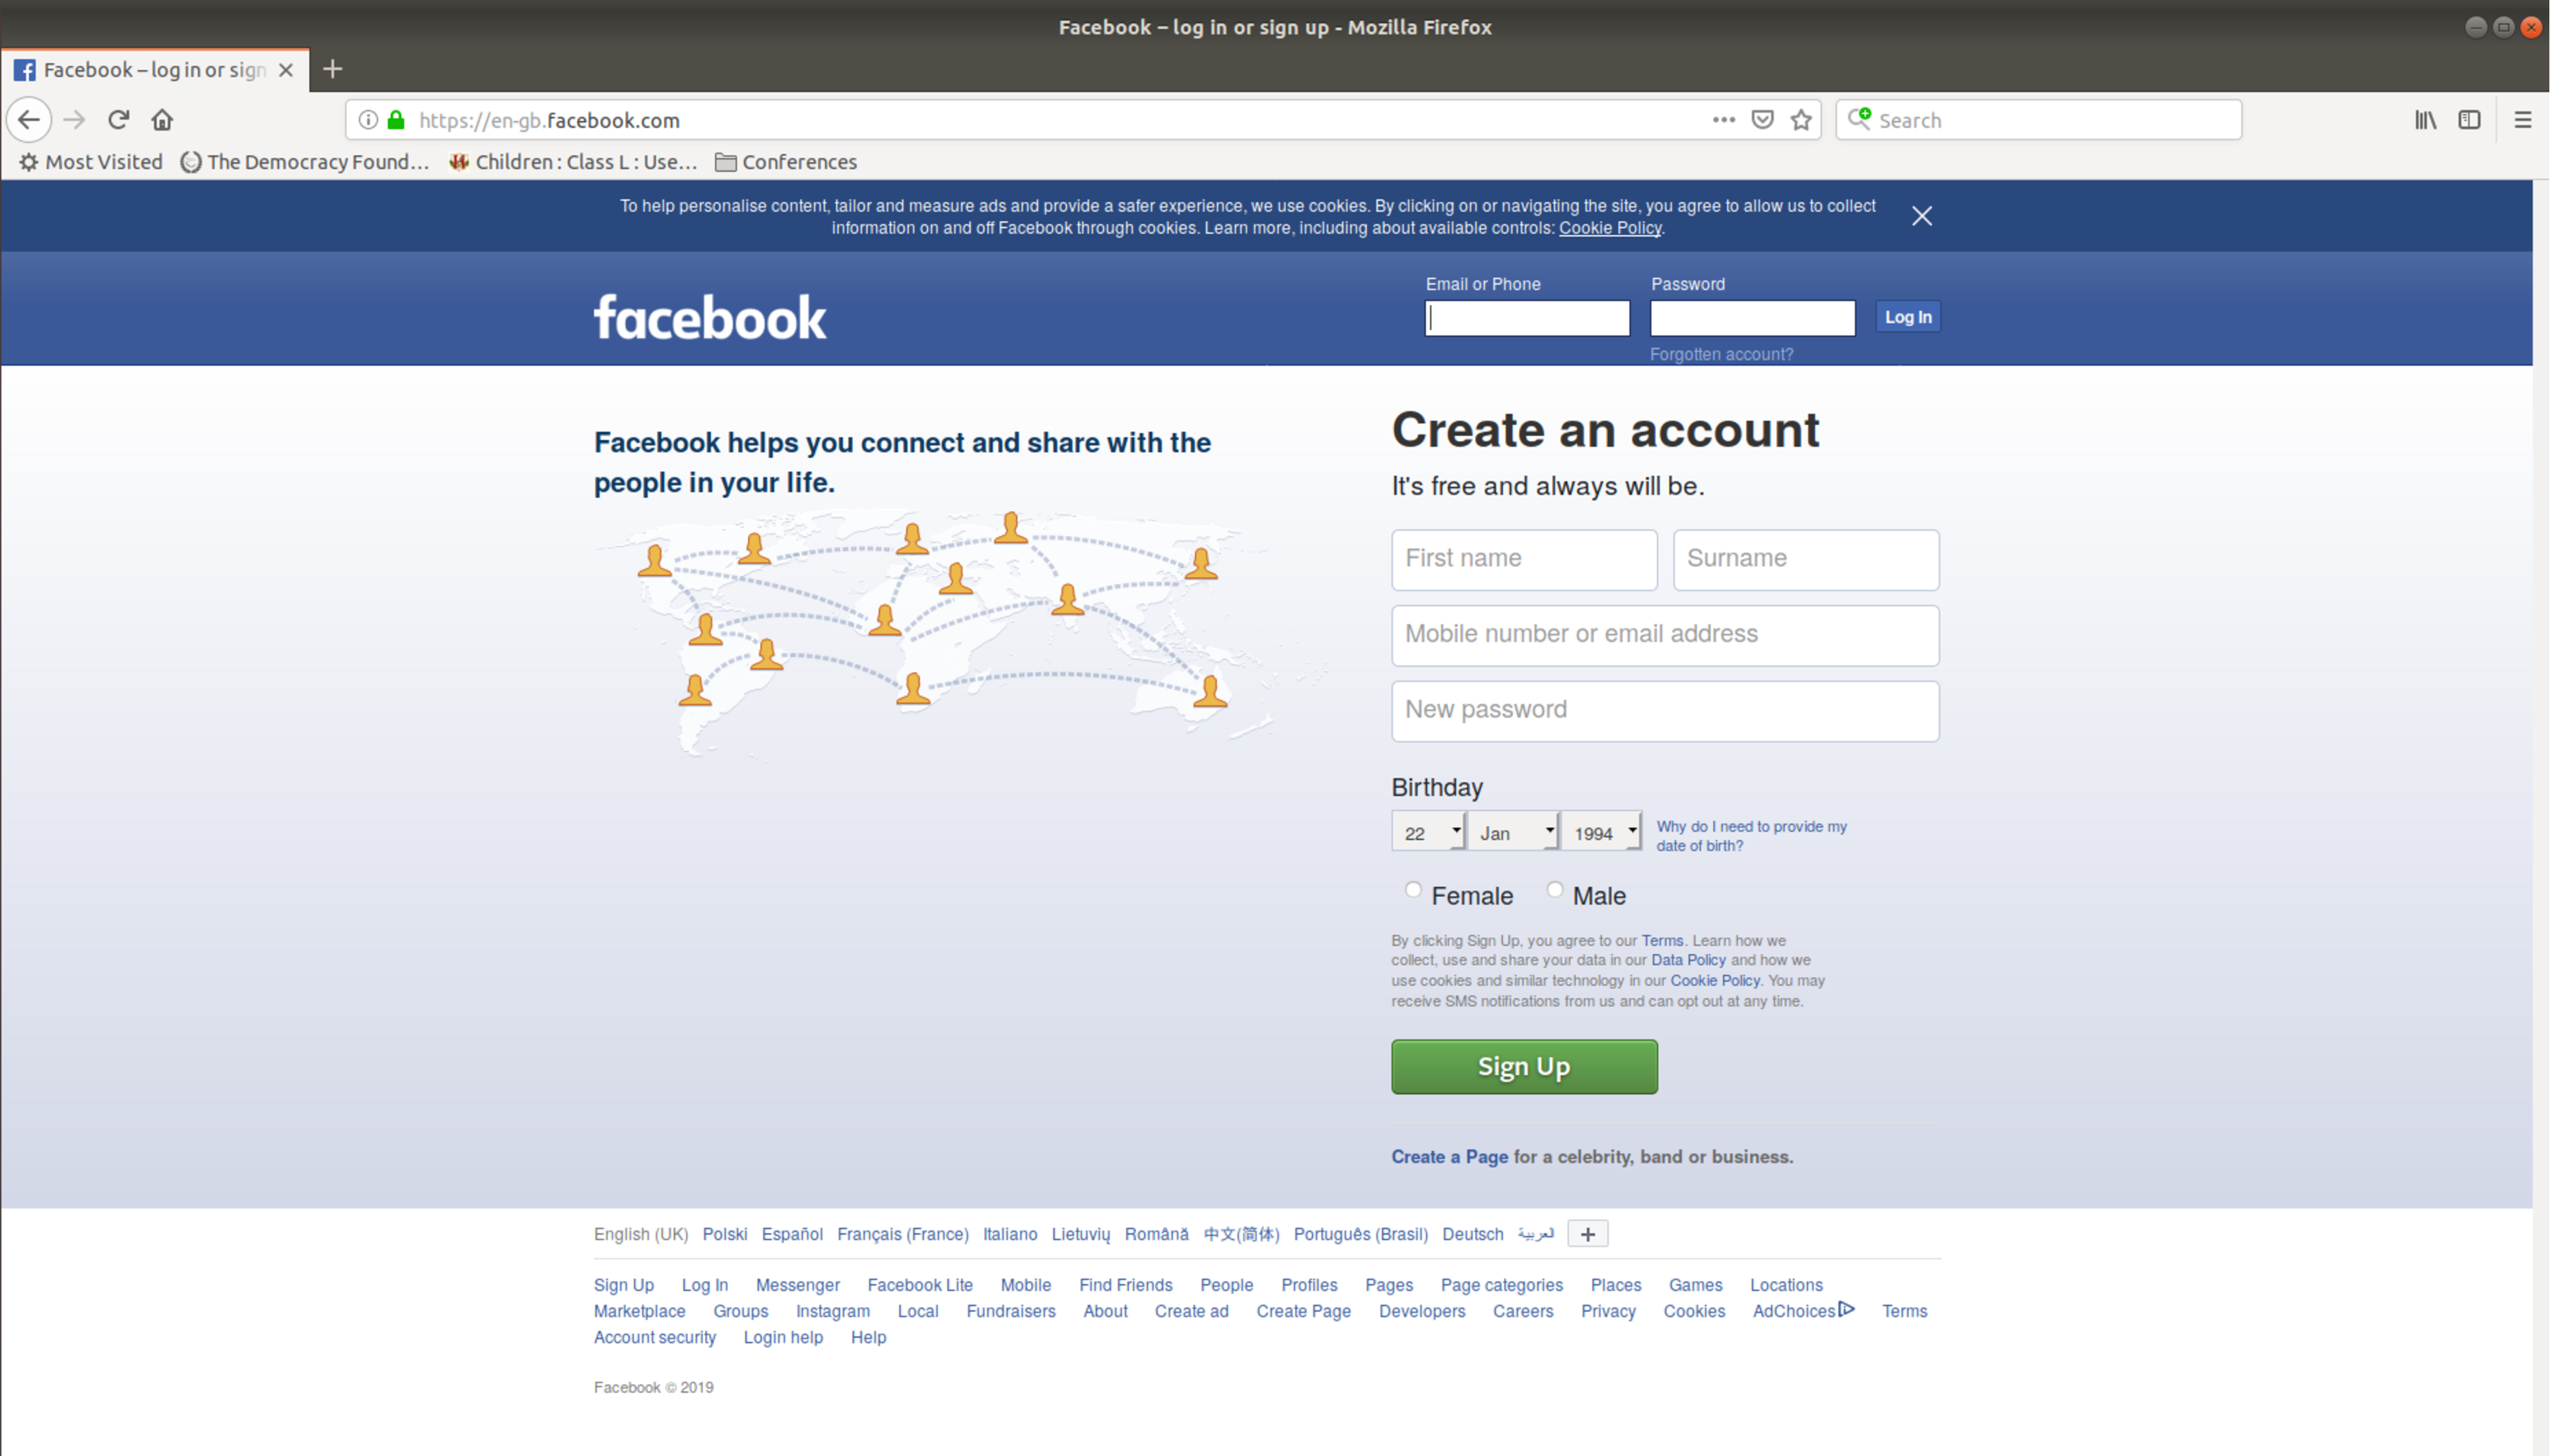
\includegraphics[scale=0.075]{Images/facebook.pdf} & 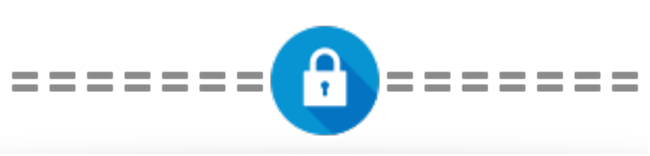
\includegraphics[scale=0.25]{Images/encrypted-channel.pdf} & 
\includegraphics[scale=0.2]{Images/laptop.pdf}
      \end{tabular}
    \end{center}
    \bigskip

  \item File protection
    \begin{center}
      
\includegraphics[scale=0.1]{Images/file-protection.pdf}
    \end{center}
  \end{itemize}
\end{frame}

\begin{frame}{Symmetric encryption schemes}
  \vspace{-0.5cm}
  \begin{block}{}
    A symmetric cipher consists of two algorithms
    \begin{itemize}
    \item encryption algorithm $E:\ \mathcal{K} \times \mathcal{M} \rightarrow \mathcal{C}$
      
    \item decryption algorithm $D:\ \mathcal{K} \times \mathcal{C} \rightarrow \mathcal{M}$
    \end{itemize}
    st. $\forall k\in\mathcal{K}$, and $\forall m\in\mathcal{M}$, $D(k, E(k, m))\ =\ m$
  \end{block}
  
  \begin{center}
    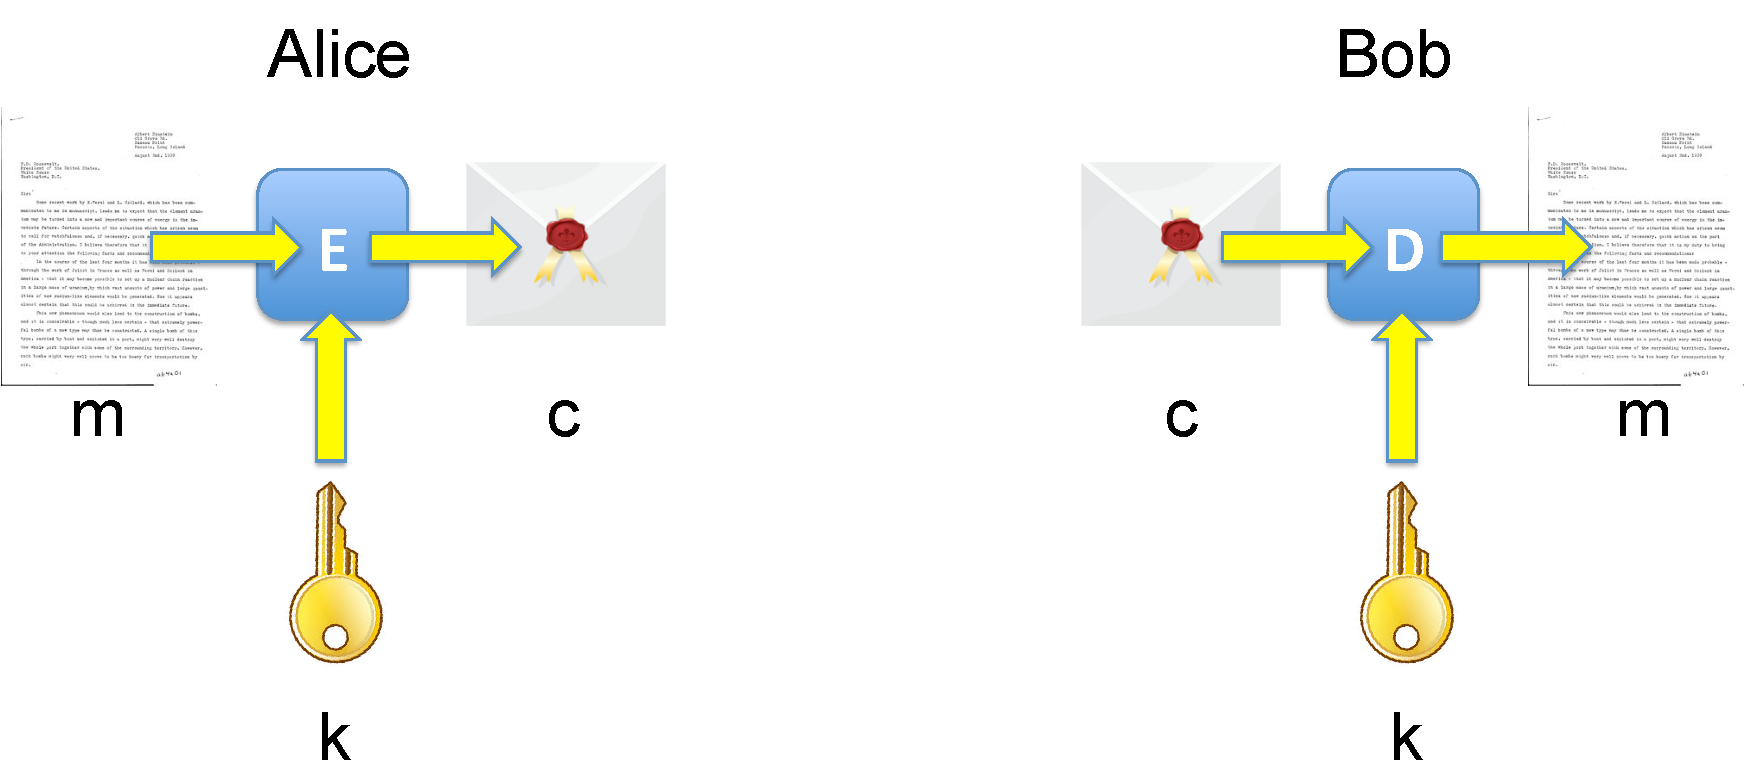
\includegraphics[scale=0.25]{Images/encryptA.pdf}
  \end{center}
  \begin{itemize}
  \item same key $k$ to encrypt and decrypt
    
  \item the key $k$ is secret: only known to Alice and Bob 
  \end{itemize}
  
\end{frame}

\begin{frame}{What is a good encryption scheme?}

  An encryption scheme is secure against a given adversary, if this adversary cannot
  
  \begin{itemize}
  \item recover the secret key $k$
  \item recover the plaintext $m$ underlying a ciphertext $c$
  \item recover any bits of the plaintext $m$ underlying a ciphertext $c$
  \item \dots    
  \end{itemize}
\end{frame}

\begin{frame}{Kerckhoff's principle}

  The architecture and design of a security system/mechanism should be made public
  \bigskip
  
  \begin{alertblock}{No security through obscurity!}
    \begin{itemize}
    \item The encryption ($E$) and decryption ($D$) algorithms are public
    \item The security relies entirely on the secrecy of the key
    \end{itemize}
  \end{alertblock}
  \bigskip

  Open design allows for a system to be scrutinised by many users, white hat hackers, academics, \emph{etc.}

  \enrouge{$\rightsquigarrow$} early discovery and corrections of flaws/vulnerabilities  
\end{frame}

\begin{frame}{Adversary's capabilities}
  \vspace{-0.5cm}
  \begin{alertblock}{}
    \begin{itemize}
    \item[$\bullet$] A cryptographic scheme is secure under some assumptions, that is against a certain type of attacker
    \item[$\bullet$] A cryptographic scheme may be vulnerable to certain types of attacks but not others
    \end{itemize}
  \end{alertblock}
  \medskip
  \pause
  
  The attacker know the encryption/decryption algorithms but may have access to :
  \begin{itemize}
  \item \Inblue{Ciphertext only attack} - some ciphertexts $c_1$, \ldots, $c_n$
    \medskip
    
  \item \Inblue{Known plaintext attack} some plaintext/ciphertext pairs $(m_1, c_1)$, \ldots, $(m_n, c_n)$ st. $c_i = E(k, m_i))$
    \medskip
    
  \item \Inblue{Chosen plaintext attack} - he has access to an encryption oracle - can maybe trick a user to encrypt messages $m_1$, \dots, $m_n$ of his choice
    \medskip

  \item \Inblue{Chosen ciphertext attack} - he has access to a decryption oracle - can maybe trick a user to decrypt ciphertexts $c_1$, \dots, $c_n$ of his choice
    \medskip

  \item unlimited, or polynomial, or realistic ($\le 2^{80}$) \Inblue{computational power}

  \end{itemize}

\end{frame}

\begin{frame}{Brute-force attack - attack on all schemes}
  \begin{itemize}
  \item Try all possible keys $k\in\mathcal{K}$ - requires some knowledge about the structure of plaintext
    \begin{center}
      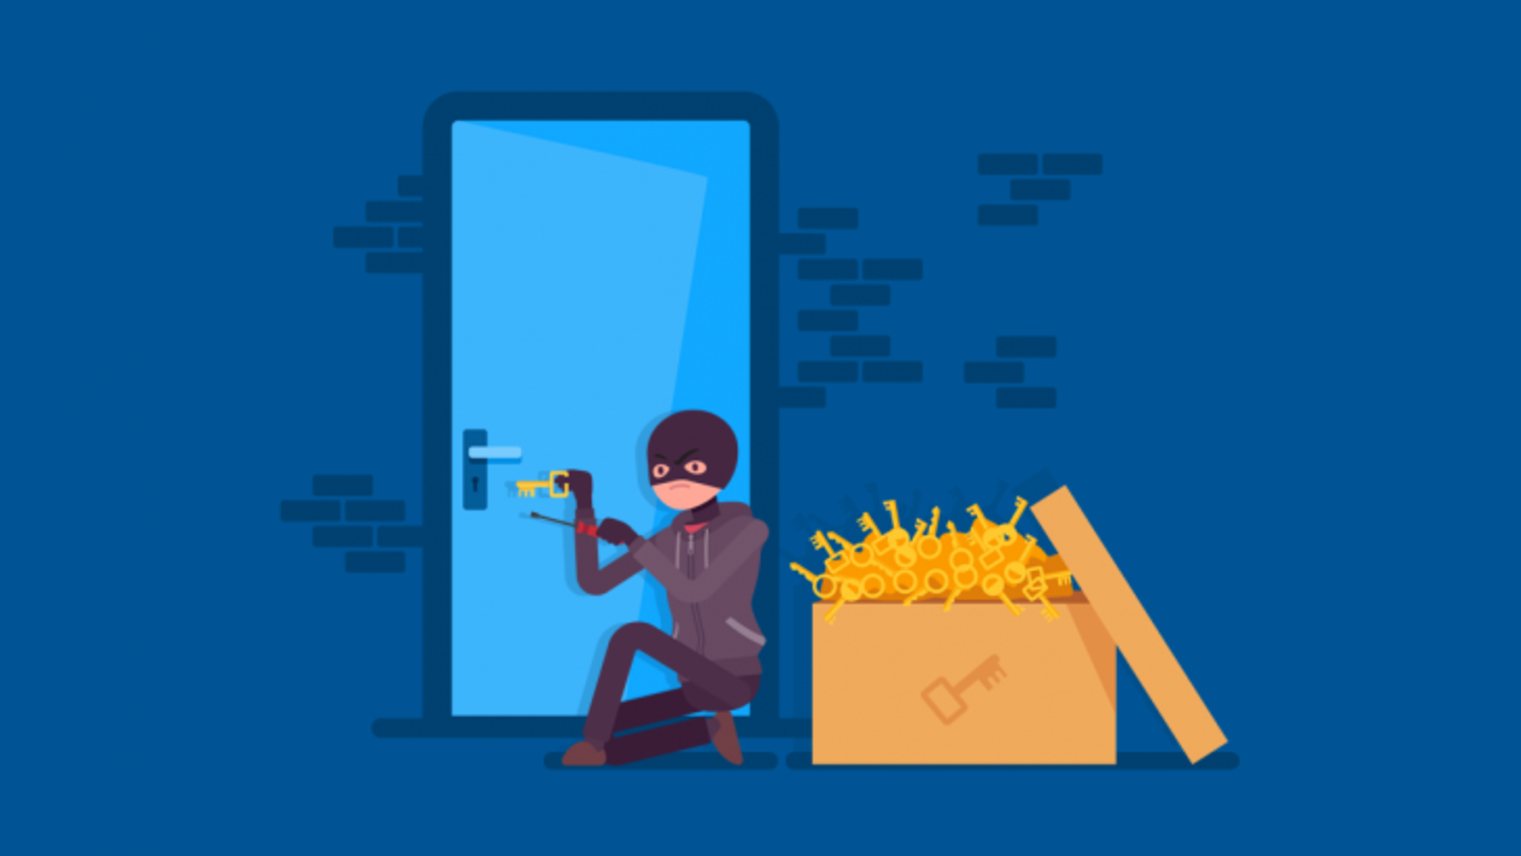
\includegraphics[scale=0.25]{Images/brute-force-attack.pdf}
    \end{center}
    \bigskip
    
  \item Making exhaustive search unfeasible:
    \begin{itemize}
    \item $\mathcal K$ should be sufficiently large, \emph{i.e.} keys
      should be sufficiently long
    \item Keys should be sampled uniformly at random from $\mathcal K$
  \end{itemize}

  \end{itemize}
\end{frame}

\begin{frame}{The One-Time Pad (OTP)}
  \pause
  \vspace{-0.5cm}
  \begin{itemize}

  \item $\Mcal\ =\ \Ccal\ =\ \Kcal\ =\ \{0, 1\}^n$
    \medskip{}
    \pause

  \item Encryption: $\forall k\in\Kcal.\ \forall m\in\Mcal.\ E(k, m) = k \oplus m$
    \pause
    \color{vert}
    \[
    \begin{array}[t]{ccccccccccccccccccccc}
      k & = & 0 & 1 & 1 & 0 & 1 & 0 & 0 & 1 \\
      m & = & 1 & 0 & 0 & 0 & 1 & 0 & 1 & 1 \\
      \hline \\
      c & = & 1 & 1 & 1 & 0 & 0 & 0 & 1 & 0
    \end{array}
    \]
    \color{black}
    \pause

  \item Decryption: $\forall k\in\Kcal.\ \forall c\in\Ccal.\ D(k, c) = k \oplus c$
    \pause
    \color{vert}
    \[
    \begin{array}[t]{ccccccccccccccccccccc}
      k & = & 0 & 1 & 1 & 0 & 1 & 0 & 0 & 1 \\
      c & = & 1 & 1 & 1 & 0 & 0 & 0 & 1 & 0 \\
      \hline \\
      m & = & 1 & 0 & 0 & 0 & 1 & 0 & 1 & 1
    \end{array}
    \]
    \color{black}
    \pause

  \item Correctness: $D(k, E(k, m)) = k \oplus (k\oplus m) = m$
  \end{itemize}
\end{frame}

\begin{frame}{Perfect secrecy}
  

  \begin{definition}
    A cipher $(E, D)$ over $(\Mcal, \Ccal, \Kcal)$ satisfies perfect secrecy if for all messages $m_1, m_2\in\Mcal$ of same length ($|m_1|=|m_2|$), and for all ciphertexts $c\in\Ccal$
    \[
    \left| Pr(E(k, m_1) = c) - Pr(E(k, m_2) = c)
    \right| \le \epsilon
    \]
    where $k \xleftarrow[]{r} \Kcal$ and $\epsilon$ is some ``negligible quantity''.
  \end{definition}

\end{frame}

\begin{frame}{OTP satisfies perfect secrecy}
    \vspace{-0.5cm}
  \begin{theorem}[Shannon 1949]
    The One-Time Pad satisfies perfect secrecy
  \end{theorem}

  \underline{Proof:} We first note that for all messages $m\in\Mcal$ and all ciphertexts $c\in\Ccal$
  \[
  \begin{array}{lcl}
    Pr(E(k, m) = c) & {=} & {\frac{\#\{k\in\Kcal:\ k\oplus m = c\}}{\#\Kcal}} \\[0.2cm]
                    & {=} & {\frac{\#\{k\in\Kcal:\ k = m\oplus c\}}{\#\Kcal}} \\[0.2cm]
                    & {=} & {\frac{1}{\#\Kcal}}
  \end{array}
  \]
  {where $k \xleftarrow[]{r} \Kcal$.}

  {Thus, for all messages $m_1, m_2\in\Mcal$, and for all ciphertexts $c\in\Ccal$}
  \[
    {\left| Pr(E(k, m_1) = c) - Pr(E(k, m_2) = c)
      \right| \le} {\left|\frac{1}{\#\Kcal} - \frac{1}{\#\Kcal}\right| = 0}
  \]

  
\end{frame}

\begin{frame}{Two-time pad attacks}
  \medskip
  
  \begin{figure}
    \centering
    \begin{tabular}[c]{ccccc}
    \begin{tabular}[c]{c}
      
\includegraphics[scale=0.3]{Images/OTP_plaintext1.pdf} \\
      $m_1$
    \end{tabular} &
    \begin{tabular}[c]{c}
      $\bigoplus$      
    \end{tabular} &
    \begin{tabular}[c]{c}
      
\includegraphics[scale=0.3]{Images/OTP_key.pdf} \\
      $k$
    \end{tabular} &
    \begin{tabular}[c]{c}
      =
    \end{tabular} &
    \begin{tabular}[c]{c}
      
\includegraphics[scale=0.3]{Images/OTP_ciphertext1.pdf} \\
      $c_1$
    \end{tabular}
    \\[3em]
    \begin{tabular}[c]{c}
      
\includegraphics[scale=0.3]{Images/OTP_plaintext2.pdf} \\
      $m_2$
    \end{tabular} &
    \begin{tabular}[c]{c}
    $\bigoplus$      
    \end{tabular} &
    \begin{tabular}[c]{c}
      
\includegraphics[scale=0.3]{Images/OTP_key.pdf} \\
      $k$
    \end{tabular} &
    \begin{tabular}[c]{c}
      =
    \end{tabular} &
    \begin{tabular}[c]{c}
      
\includegraphics[scale=0.3]{Images/OTP_ciphertext2.pdf} \\
      $c_2$
    \end{tabular}\\[2em]
    \hline\\
    \begin{tabular}[c]{c}
      
\includegraphics[scale=0.3]{Images/OTP_ciphertext1.pdf} \\
      $c_1$
    \end{tabular} &
    \begin{tabular}[c]{c}
    $\bigoplus$      
    \end{tabular} &
    \begin{tabular}[c]{c}
      
\includegraphics[scale=0.3]{Images/OTP_ciphertext2.pdf} \\
      $c_2$
    \end{tabular} &
    \begin{tabular}[c]{c}
      =
    \end{tabular} &
    \begin{tabular}[c]{c}
      
\includegraphics[scale=0.3]{Images/OTP_plaintext12.pdf} \\
      $m_1\oplus m_2$
    \end{tabular}
  \end{tabular}
  \caption*{Source: Cryptosmith and David Lowry-Duda, \url{crypto.stackexchange.com/}}
\end{figure}

\end{frame}

\begin{frame}{Limitations of OTP}
  \pause

  \begin{itemize}

  \onslide<2->{\item Key-length!
  \begin{itemize}
    \onslide<2->{\item The key should be as long as the plaintext}
  \end{itemize}}
  \bigskip{}
  
  \onslide<3->{\item Getting true randomness!
  \begin{itemize}
    
    \onslide<3->{\item} The key should not be guessable from an attacker
    \onslide<3->{\item} If the key is not truly random, frequency analysis might again be possible
    
  \end{itemize}}
  \bigskip{}

  \onslide<4->{\item Perfect secrecy does not capture all possible attacks
    \begin{itemize}
      \onslide<5->{\item \enrouge{OTP is subject to two-time pad attacks}}
      
      \onslide<5->{\enrouge{given $m_1 \oplus k$ and $m_2 \oplus k$, we can compute $m_1\oplus m_2 = (m_1 \oplus k)\oplus(m_2\oplus k)$}}

      \onslide<5->{\enrouge{English has enough redundancy s.t. $m_1\oplus m_2 \rightarrow m_1, m_2$}}
      \medskip{}

      
      \onslide<6->{\item \enrouge{OTP is malleable}}

      \color{rouge}
      \onslide<6->{given the ciphertext $c = E(k, m)$ with $m = to\ bob: m_0$, it is possible to compute the ciphertext $c' = E(k, m')$ with $m' = to\ eve: m_0$ $c':= c\oplus "to\ bob: 00\dots00"\oplus "to\ eve: 00\dots00"$}
      \color{black}
      
    \end{itemize}
  }
  
  \end{itemize}

\end{frame}

\covertopicname{Stream ciphers}
\author{}
\date{}

\begin{frame}
  \titlepage
\end{frame}

\begin{frame}
  \frametitle{Stream ciphers}

  \begin{itemize}
  \item Goal: make the OTP practical
    \medskip{}
    \pause
  \item Idea: use a pseudorandom key rather than a really random key
    \pause
    \begin{itemize}
    \item The key will not really be random, but will look random
      \pause
    \item The key will be generated from a key seed using a Pseudo-Random Generator (PRG)

      $G:\ \{0, 1\}^s \rightarrow \{0, 1\}^n$ with $s<<n$
    \end{itemize}
    \medskip{}
    \pause
  \item Encryption using a PRG $G$: $E(k, m) = G(k) \oplus m$
    \medskip{}
    \pause
  \item Decryption using a PRG $G$: $D(k, c) = G(k) \oplus c$
    \medskip{}
    \pause{}

  \item \enrouge{Stream ciphers are subject to two-time pad attacks}
    \medskip{}
    \pause{}

  \item \enrouge{Stream ciphers are malleable}
  \end{itemize}
 
\end{frame}

\begin{frame}{RC4}

  \begin{itemize}
  \item Stream cipher invented by Ron Rivest in 1987 
    \pause
    \medskip{}
    
  \item Consists of 2 phases:
    \begin{center}
      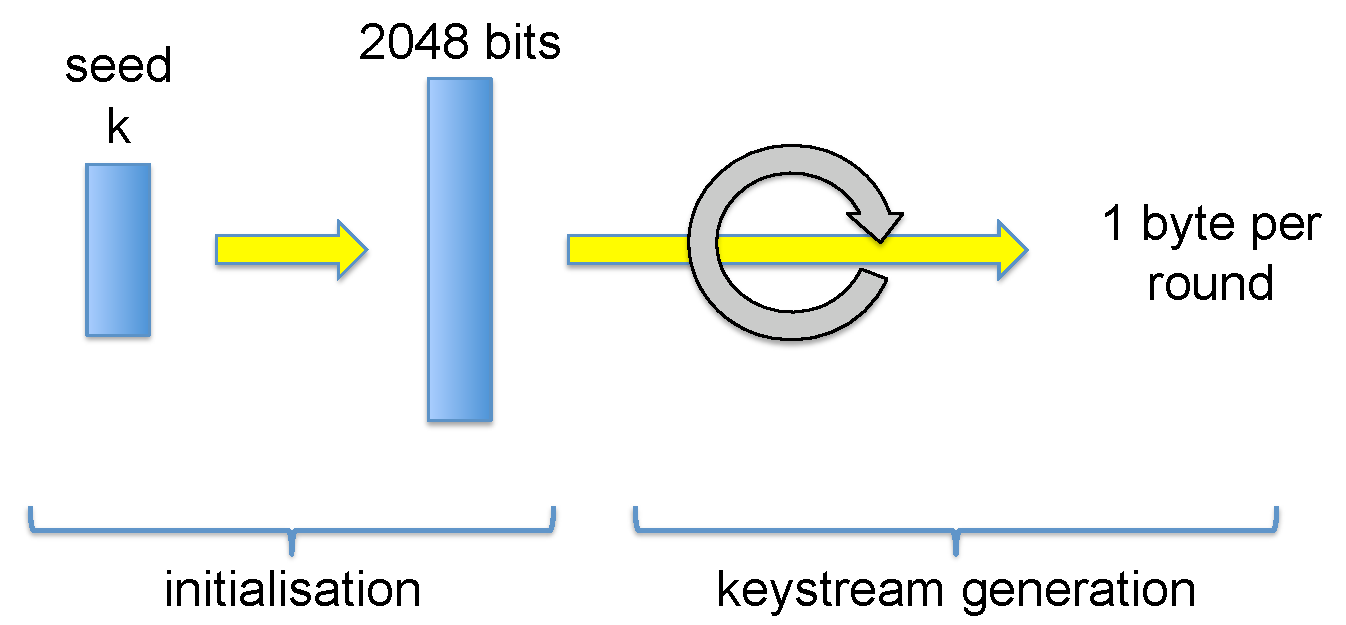
\includegraphics[scale=0.25]{Images/RC4.pdf}
    \end{center}
    \pause

  \item Used in HTTPS and WEP
    \medskip{}
    \pause

  \item Weaknesses of RC4:
    \begin{itemize}
    \item \enrouge{first bytes are biased}
      
      \enrouge{$\longrightarrow$ drop the first to 256 generated bytes}
      \pause

    \item \enrouge{subject to related keys attacks}

      \enrouge{$\longrightarrow$ choose randomly generated keys as seeds}
    \end{itemize}
  \end{itemize}

\end{frame}

\begin{frame}
  \frametitle{WEP uses RC4}

  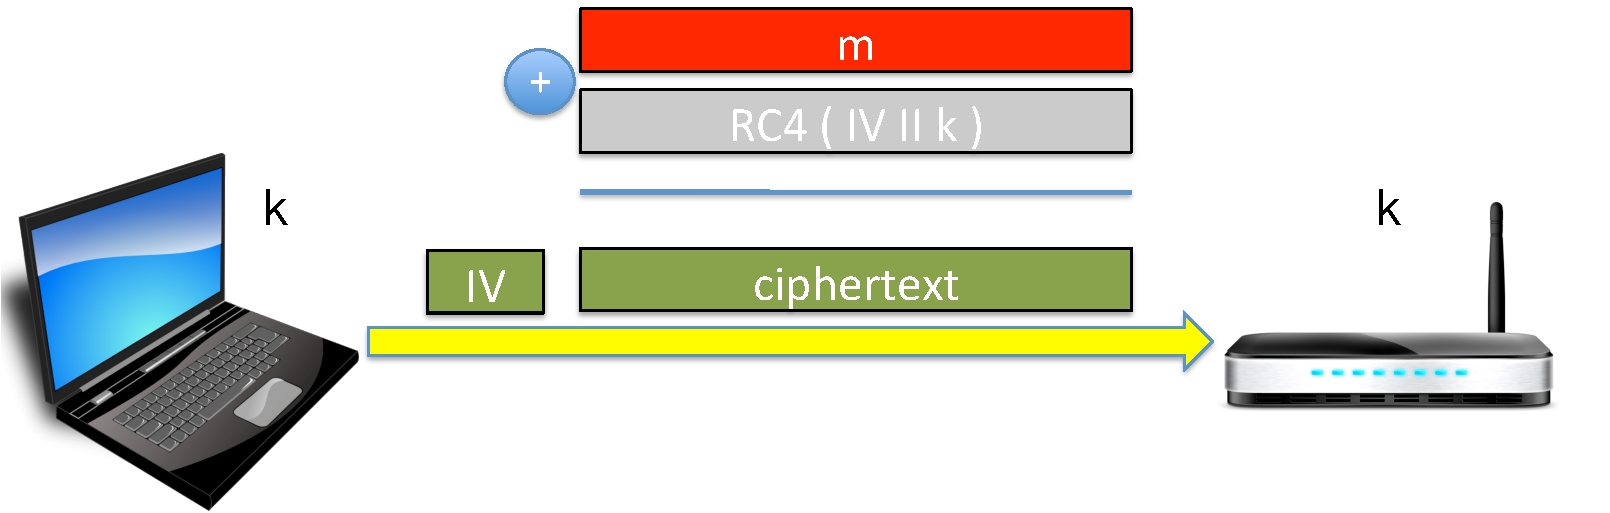
\includegraphics[scale=0.4]{Images/WEP.pdf}
  \bigskip{}

  Initialisation Vector (IV): 24-bits long string
  
\end{frame}

\begin{frame}
  \frametitle{Weaknesses of WEP}

  \pause
  \begin{itemize}
  \item two-time pad attack: IV is 24 bits long, so the key is reused after at most $2^{24}$ frames

    \envert{$\longrightarrow$ use longer IVs}
    \medskip{}
    \pause
  \item Fluhrer, Mantin and Shamir (FMS) attack (related keys attack): 
  
    -\begin{tabular}[t]{l}
      the keys only differ in the 24 bits IV
    \end{tabular}
    
    -\begin{tabular}[t]{l}
      first bytes of key stream known because standard headers \\
      are always sent
    \end{tabular}
    
    \mbox{-\begin{tabular}[t]{l}
      for certain IVs knowing $m$ bytes of key and keystream means \\
      you can deduce byte $m + 1$ of key
    \end{tabular}}
      
    \envert{$\longrightarrow$ instead of using related IVs, generate IVs using a PRG}
    
    \pause
     \envert{$\longrightarrow$ or even better generate message specific seeds using a PRG}

    \end{itemize}
    \medskip{}

\end{frame}

\begin{frame}
  \frametitle{Weaknesses of TLS}
    \vspace{-0.5cm}

  \begin{center}
    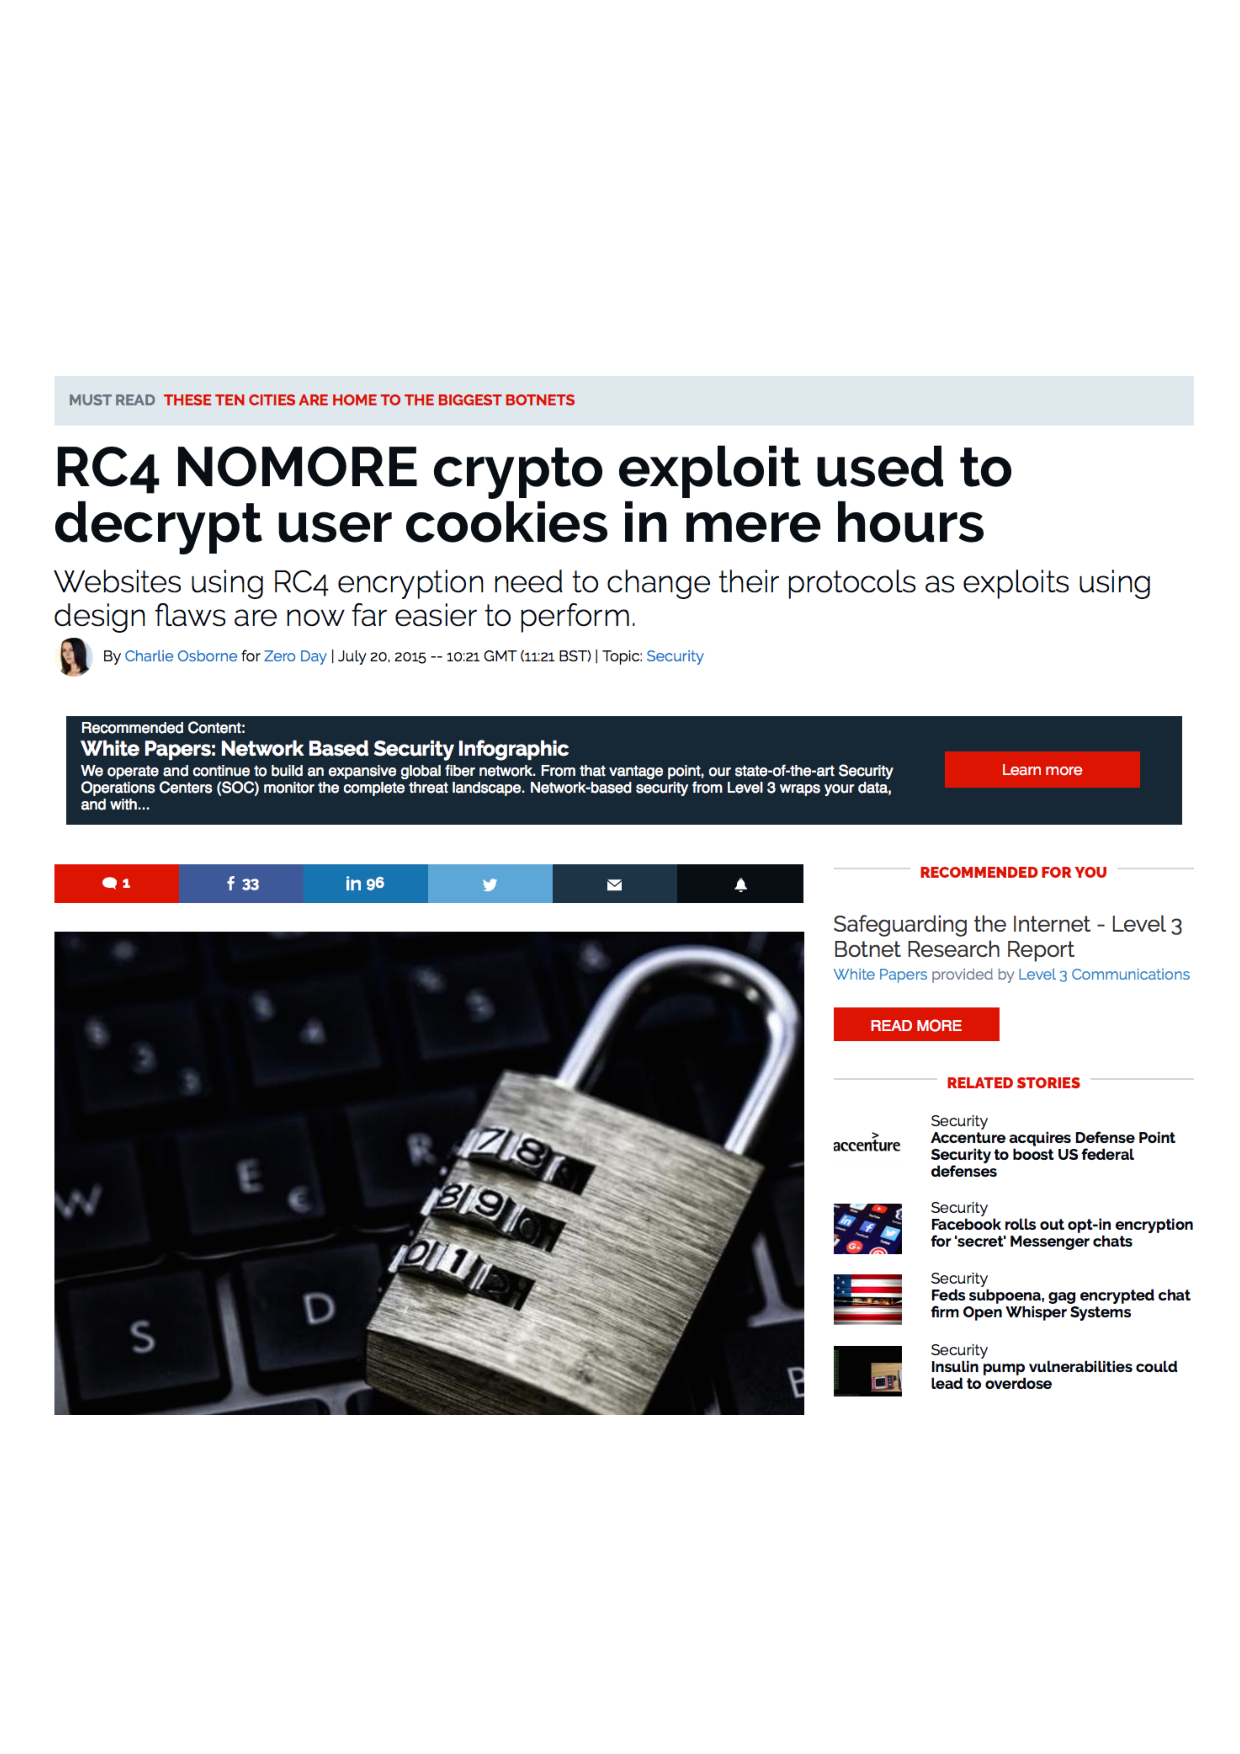
\includegraphics[scale=0.4]{Images/rc4-tls-attack.pdf}
  \end{center}

\end{frame}

\begin{frame}
  \frametitle{Android BitCoin attack}
  \vspace{-0.5cm}
  \begin{center}
    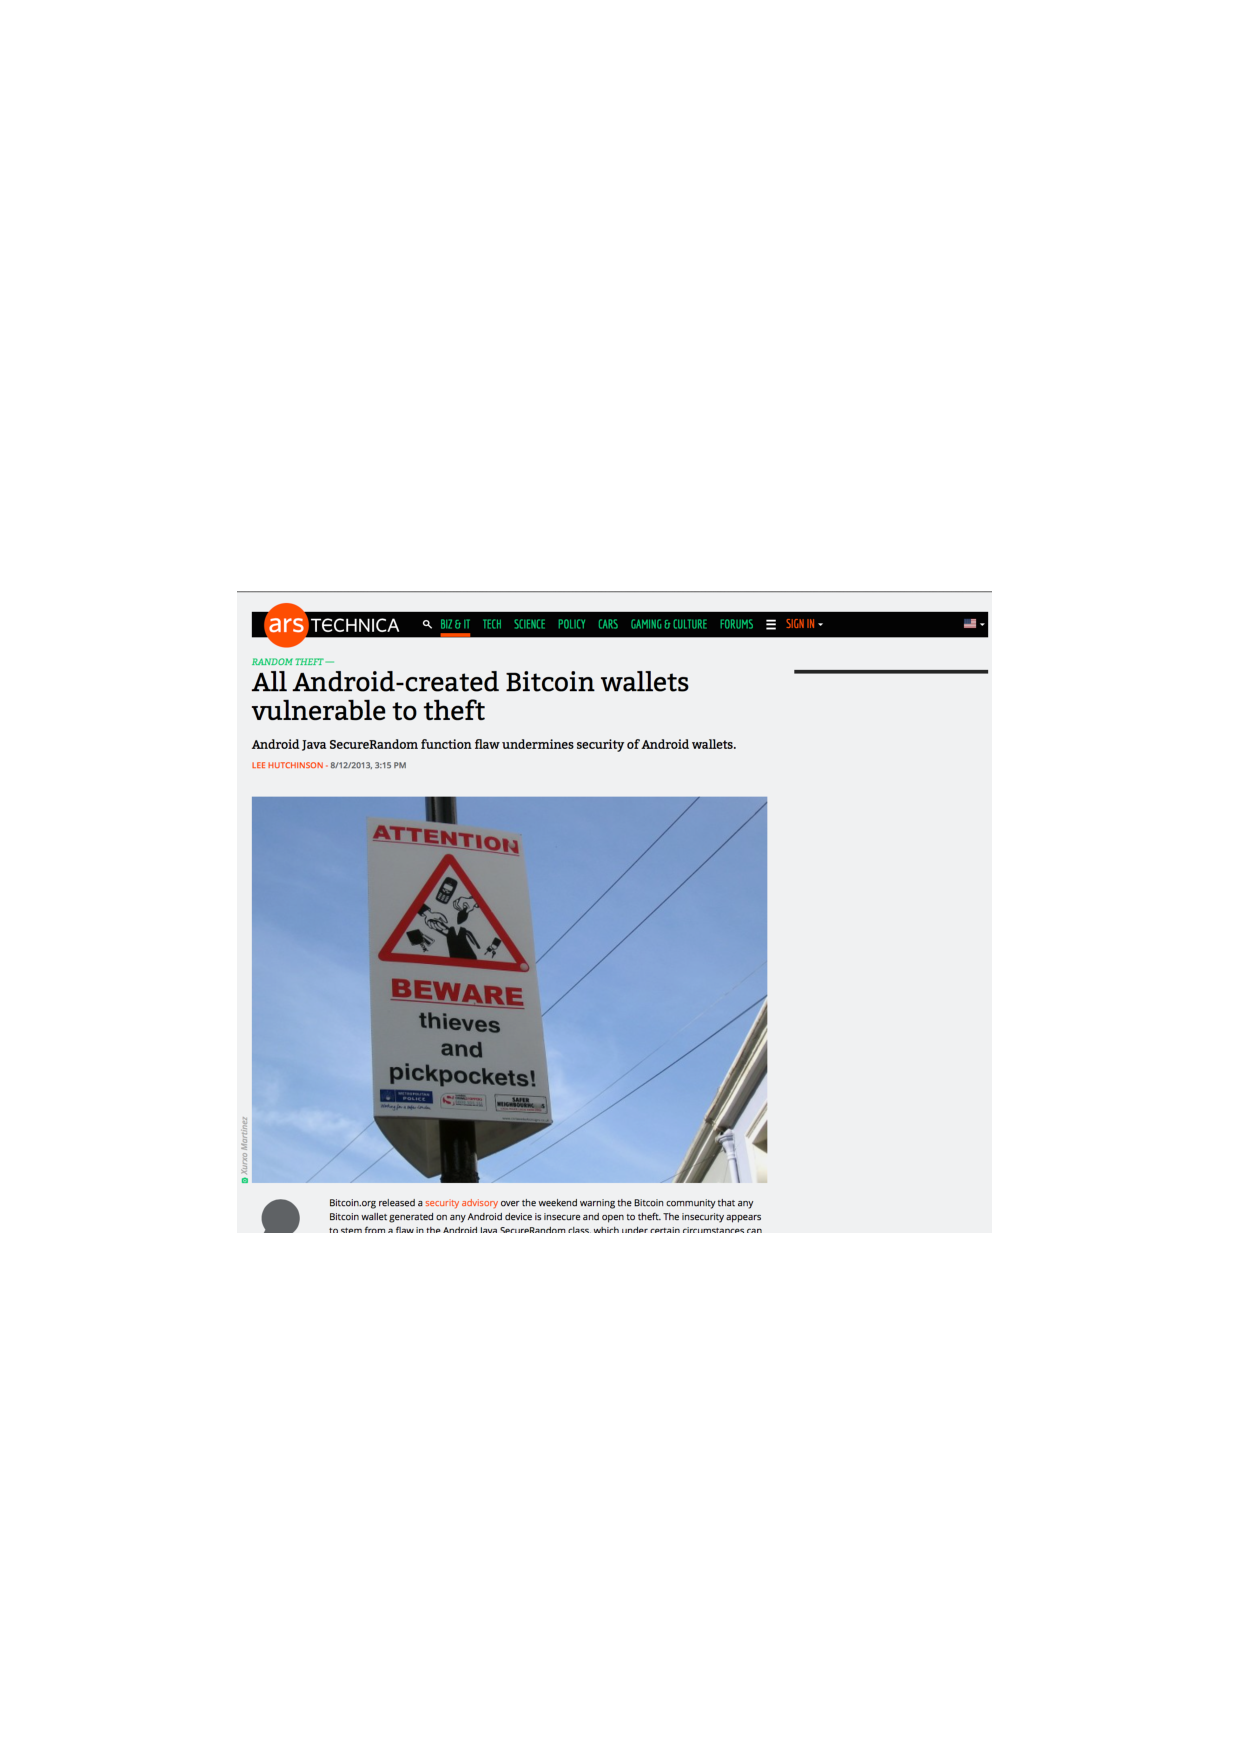
\includegraphics[scale=0.65]{Images/AndroidBitcoinAttack.pdf}
  \end{center}


\end{frame}

\begin{frame}
  \frametitle{Modern stream ciphers}

  {\bf Project eStream}: project to ``identify new stream ciphers suitable for widespread adoption'', organised by the EU ECRYPT network

  $\longrightarrow$\begin{tabular}[t]{l}
    HC-128, Rabbit, Salsa20/12, SOSEMANUK, \\
    Grain v1, MICKEY 2.0, Trivium
  \end{tabular}
  \bigskip{}
  \pause

  \begin{block}{Conjecture}
    These eStream stream ciphers are ``secure''
  \end{block}

\end{frame}

\begin{frame}
  \frametitle{Concluding remarks on Stream Ciphers}
  \pause

  \begin{itemize}
  \item Perfect secrecy does not capture all possible attacks.
    
    \enrouge{$\longrightarrow$ need for different security definition}
    \medskip
    \pause

  \item Theorem (Shannon 1949) Let $(E, D)$ be a cipher over $(\Mcal, \Ccal, \Kcal)$. If $(E, D)$ satisfies perfect secrecy, then the keys should be at least as long as the plaintexts ($|\Mcal|\le |\Kcal| $).

    $\Rightarrow$ Stream ciphers do not satisfy perfect secrecy because the keys in $\Kcal$ are smaller than the messages in $\Mcal$

    \enrouge{$\longrightarrow$ need for different security definition}
    \medskip
    \pause

  \item The design of crypto primitives is subtle and error prone.

    \enrouge{$\longrightarrow$ use standardised publicly know primitives}
    \medskip
    \pause
    
  \item Crypto primitives are secure under a precisely defined threat model.

    \enrouge{$\longrightarrow$ respect the security assumptions of the crypto primitives}
    \medskip
    \pause

  \item Many attacks due to poor implementations of cryptography
  \end{itemize}

\end{frame}

\covertopicname{Block ciphers}
\date{}
\author{}

\begin{frame}
  \maketitle
\end{frame}

\begin{frame}
  
  \frametitle{Block ciphers}

  A block cipher with parameters $k$ and $\ell$ is a pair of deterministic algorithms $(E, D)$ such that
  \begin{itemize}
  \item Encryption $E: \{0, 1\}^k \times \{0, 1\}^\ell \rightarrow \{0, 1\}^\ell$
  \item Decryption $D: \{0, 1\}^k \times \{0, 1\}^\ell \rightarrow \{0, 1\}^\ell$
  \end{itemize}
  \bigskip{}

  \envert{Examples:}

  \hspace{1cm}\envert{3DES: $\ell=64$, $k=168$}

  \hspace{1cm}\envert{AES: $\ell=128$, $k=128, 192, 256$}
\end{frame}

\begin{frame}

  \frametitle{Data Encryption Standard (DES)}

  \begin{itemize}

  \item Early 1970s: Horst Feistel designs Lucifer at IBM 
  
  $k = 128$ bits, $\ell = 128$ bits 
  \bigskip{}

  \item 1973: NBS calls for block cipher proposals. 

    $\longrightarrow$ IBM submits a variant of Lucifer.  
  \bigskip{}
 
  \item 1976: NBS adopts DES as a federal standard 

    $k = 56$ bits, $\ell = 64$ bits
    \bigskip{}
    
  \item 1997: DES broken by exhaustive search
    \bigskip{}
    
  \item 2001: NIST adopts AES to replace DES

    $k = 128, 192, 256$ bits, $\ell = 128$ bits
  \end{itemize}
  \bigskip{}

  Was widely deployed in banking (ATM machines) and commerce - now deprecated

\end{frame}

\begin{frame}

  \frametitle{Attacks on DES}

  \pause

  \begin{itemize}
  \item {\bf Exhaustive search:} it takes $2^{56}$ to do an exhaustive search over the key space

    $\longrightarrow$ COBACOBANA (120 FPGAs, $\sim$ 10K\$): 7 days 
    \bigskip{}
    \pause

  \item {\bf Linear cryptanalysis:} found affine approximations to DES
    $\longrightarrow$\begin{tabular}[t]{l}
      can find 14 key bits in time $2^{42}$ \\
      brute force the remaining 56-14=42 in time $2^{42}$ \\
      $\Rightarrow$ total attack time $\approx 2^{43}$
    \end{tabular}
  \end{itemize}
  \bigskip{}
  \pause
  
  \enrouge{$\Rightarrow$ DES is badly broken! Do not use it in new projects!!}

\end{frame}

\begin{frame}

  \frametitle{Triple DES (3DES)}
  
  \begin{itemize}
  \item Goal: build on top of DES a block cipher resistant against exhaustive search attacks
    \medskip{}
    \pause

  \item Used in bank cards and RFID chips
    \medskip{}
    \pause

  \item Let $DES = (E_{DES}, D_{DES})$. We build $3DES = (E_{3DES}, D_{3DES})$ as follows
    \smallskip{}
    \pause
    \begin{itemize}
    \item $E_{3DES}: (\{0, 1\}^k)^3 \times \{0, 1\}^\ell \rightarrow \{0, 1\}^\ell $

      $E_{3DES}((K_1, K_2, K_3), M) = E_{DES}(K_1, D_{DES}(K_2, E_{DES}(K_3, M)))$
\pause
      $\longrightarrow\ K_1 = K_2 = K_3 \Rightarrow DES$
      \smallskip{}
      \pause

    \item $D_{3DES}: (\{0, 1\}^k)^3 \times \{0, 1\}^\ell \rightarrow \{0, 1\}^\ell $

      $D_{3DES}((K_1, K_2, K_3), C) = D_{DES}(K_3, E_{DES}(K_2, D_{DES}(K_1, C)))$
      \medskip{}
      \pause
    \end{itemize}

  \item[] \enrouge{$\longrightarrow$ 3 times as slow as DES!!}
    \medskip{}
    \pause

  \item key-size = $3\times 56=168$ bits
    
    $\Rightarrow$ Exhaustive search attack in $2^{168}$
    \medskip{}
    \pause
  \item simple (meet-in-the-middle) attack in time $2^{118}$
  \end{itemize}

\end{frame}

\begin{frame}

  \frametitle{What about double DES (2DES)?}
  \pause

  \begin{itemize}
  \item $E_{2DES}((K_1, K_2), M) = E_{DES}(K_1, E_{DES}(K_2, M))$

    \begin{center}
      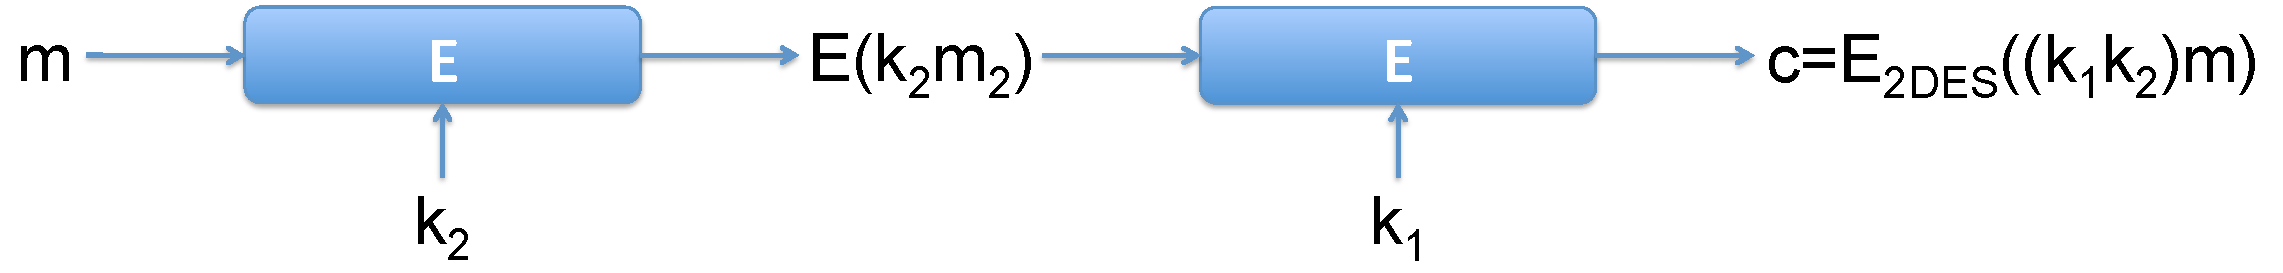
\includegraphics[scale=0.25]{Images/2DES.pdf}
    \end{center}
    \pause
    $\Rightarrow
    \begin{array}[t]{ll}
      \text{For } m \text{ and } c \text{ such that } E_{2DES}((k_1, k_2), m) = c \text{ we have} \\
      \text{that } E_{DES}(k_2, m) = D_{DES}(k_1, c)
    \end{array}
    $

    \medskip{}
    \pause
  \item 2DES admits a meet-in-the-middle attack that reduces the time for key recovery from $2^{112}$ for an exhaustive search to $2^{63}$. Given $M = (m_1, \dots, m_{10})$ and $C = (E_{2DES}((k_1, k_2), m_1), \dots, E_{2DES}((k_1, k_2), m_{10}))$
    \pause
    \[
    \hspace{-0.25cm}\begin{array}{l}
      \left.
        \begin{array}[c]{l}
          \text{- For all possible } k_2{, compute\, } E_{DES}(k_2, M) \\
          \text{- Sort table according to the resulting } E_{DES}(k_2, M)
        \end{array}
      \right\} 2^{56}\text{log}(2^{56})
      \pause
      \\
      \left.
        \begin{array}[c]{l}
          \text{- For each possible } k_1{, compute\, } D_{DES}(k_1, C) \\
          \text{- Look up in the table if } D_{DES}(k_1, C) = E_{DES}(k_2, M)
        \end{array}
      \right\} 2^{56}\text{log}(2^{56}) \\
      \pause
      \hfill\enrouge{\Rightarrow \text{ time }< 2^{63}}
    \end{array}
    \]
    \pause

  \item Similar attack on 3DES in time $2^{118}$
  \end{itemize}

\end{frame}


\begin{frame}

  \frametitle{The Advanced Encryption Standard (AES)}

  \begin{itemize}
  \item Goal: replace 3DES which is too slow (3DES is 3 times as slow as DES)
    \bigskip{}
  \item 2001: NIST adopts Rijndael as AES
    \bigskip{}
  \item Block size $\ell = 128$ bits, Key size $k=128, 192, 256$ bits
  
  \end{itemize}

\end{frame}

\begin{frame}

  \frametitle{AES: encryption circuit}

  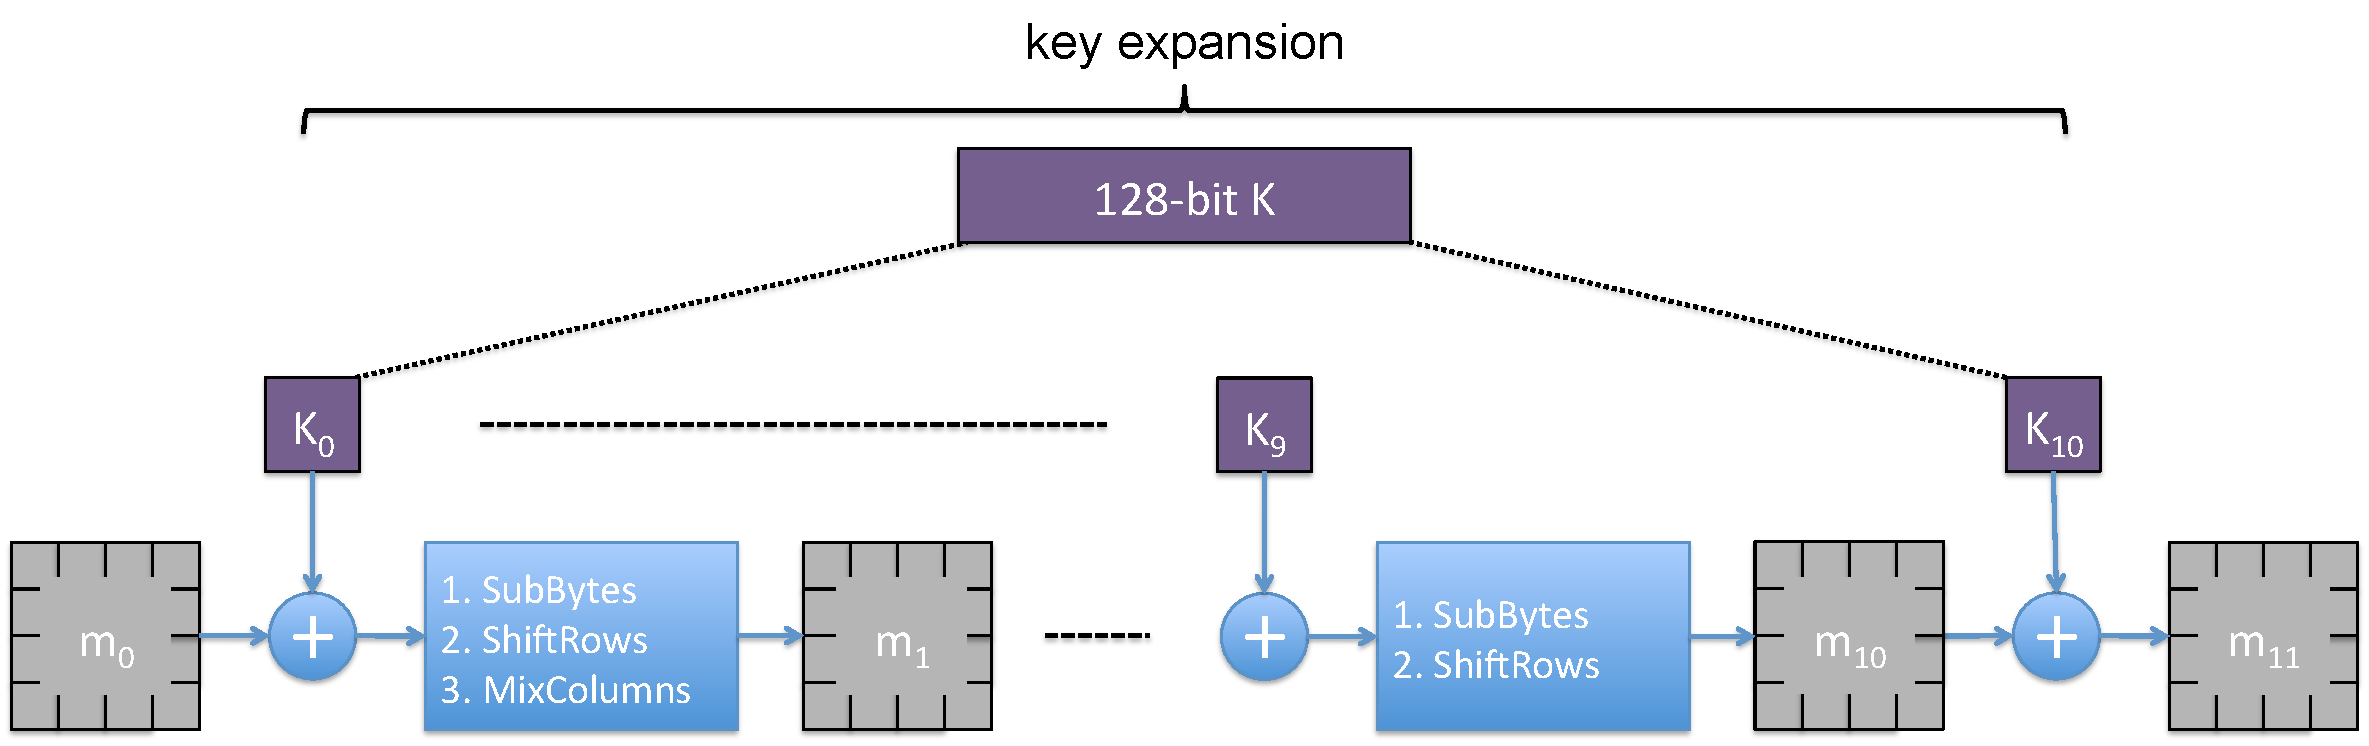
\includegraphics[scale=0.275]{Images/AES.pdf}
  \bigskip{}

  \begin{itemize}
  \item $m_i:\ 4\times 4$ byte matrix, $K_i$: 128-bit key
  \item $m_0$: plaintext, $m_{11}$: ciphertext
  \item at the last round MixColumns is not applied
  \end{itemize}

  
\end{frame}

\begin{frame}

  \frametitle{Attacks on AES}

  \begin{itemize}
  \item {\bf Related-key attack} on the 192-bit and 256-bit versions of AES: exploits the AES key schedule [A. Biryukov, D. Khovratovich (2009)]

    \enrouge{$\longrightarrow$ key recovery in time $\sim 2^{99}$}
    \bigskip{}

  \item First {\bf key-recovery attack} on full AES [A. Bogdanov, D. Khovratovich, C. Rechberger (2011)]

    \enrouge{$\longrightarrow$ 4 times faster than exhaustive search}
  \end{itemize}
  \pause
  \bigskip{}

  \enrouge{$\Rightarrow$
    \begin{tabular}[t]{l}
      Existing attacks on AES-128 are still not practical, but \\
      should use AES-192 and AES-256 in new projects!
    \end{tabular}
  }

\end{frame}

\covertopicname{Using block ciphers}
\date{}
\author{}

\begin{frame}
  \maketitle
\end{frame}

\begin{frame}
  \frametitle{Goal}

  \begin{block}{}
    Encrypt $M$ using a block cipher operating on blocks of length $\ell$ when \enrouge{$|M|\not=\ell$}
  \end{block}
\end{frame}

\begin{frame}
  \frametitle{Padding - $|M| \le \ell$}

  \begin{itemize}
  \item \enbleu{Bit padding -} append a \emph{set bit} ('1') at the end of message, and then append as many \emph{reset bits} ('0') required

    \scriptsize

    \envert{\underline{Example:} padding a 52-bits message for a 64-bits block:}

    \mbox{\envert{11010011 01010110 10010000 00111010 10110101 01011010 1111{\bf 1000 00000000}}}

    \envert{padding a $64$-bits message $M$ for 64-bits blocks requires adding a padding block:}

    \mbox{\envert{M$|${\bf 10000000 00000000 00000000 00000000 00000000 00000000 00000000 00000000}}}
    \medskip{}
    \pause
    \normalsize
    
  \item \enbleu{ANSI X.923 - } byte padding - pad with zeros, the last byte defines the number of padded bytes

    \scriptsize

    \envert{\underline{Example:} padding a 4-bytes message for 8-bytes blocks:}
    
    \envert{DD DD DD DD {\bf 00 00 00 04}}

    \envert{padding a $8k$-bytes messages for 8-bytes blocks requires adding a padding block:}

    \envert{DD DD DD DD DD DD DD DD $|$ {\bf 00 00 00 00 00 00 00 08}}
    \medskip{}
    \pause

    \normalsize
 
  \item \enbleu{PKCS\#7 - } byte padding - the value of each added byte is the total number of padding bytes. The padding will be
    01, or 02 02, or 03 03 03, or 04 04 04 04, \emph{etc.}

    \scriptsize

    \envert{\underline{Example:} padding a 4-bytes message for 8-bytes blocks:}

    \envert{DD DD DD DD {\bf 04 04 04 04}}

    \envert{padding a $8$-bytes message for 8-bytes blocks requires adding a padding block:}

    \envert{DD DD DD DD DD DD DD DD $|$ {\bf 08 08 08 08 08 08 08 08}}

    \normalsize

  \end{itemize}

\end{frame}

\begin{frame}

  \frametitle{Electronic Code Book (ECB) mode}

  $(E, D)$ a block cipher.
  \pause
  \bigskip{}

  To encrypt message $M$ under key $K$ using ECB mode: 
  \pause

  \begin{itemize}
  \item $M$ is padded:

    \hspace{1cm}$\Rightarrow\ M' = M || P$ such that $|M'| = m\times \ell$
    \pause
    \medskip{}
    
  \item $M'$ is broken into $m$ blocks of length $\ell$

    \hspace{1cm}$\Rightarrow\ M'\ = M_1\ ||\ M_2\ ||\ \dots\ ||\ M_m$
    \pause
    \medskip{}

  \item Each block $M_i$ is encrypted under the key $K$ using the block cipher

    \hspace{1cm}$\Rightarrow\ C_i = E(K, M_i)$ for all $i\in\{1, \dots, m\}$
    \pause
    \medskip{}

  \item The ciphertext corresponding to $M$ is the concatenation of the $C_i$s

    \hspace{1cm}$\Rightarrow\ C\ = C_1\ ||\ C_2\ ||\ \dots\ ||\ C_m$
  \end{itemize}

\end{frame}

\begin{frame}

  \frametitle{Weakness of ECB}
  \pause

  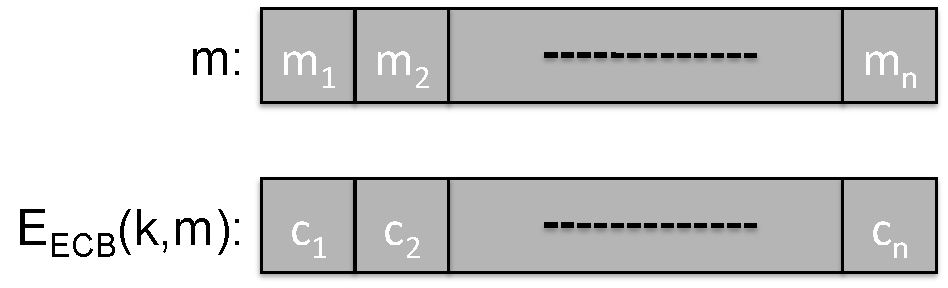
\includegraphics[scale=0.5]{Images/ECB.pdf}
  \pause
  \bigskip{}
  \bigskip{}
  \bigskip{}
  
  \enrouge{Problem: $\forall i,j.\ m_i = m_j\ \Rightarrow\ c_i= E(k, m_i) = E(k, m_j) = c_j$}
  \medskip{}
  
  \quad \quad \enrouge{$\Rightarrow$ Malleable and weak to frequency analysis!}

  \bigskip{}
  
\end{frame}

\begin{frame}

  \frametitle{Weakness of ECB in pictures}
  \vspace{-0.5cm}
  \begin{tabular}{cc}
    \onslide<1->{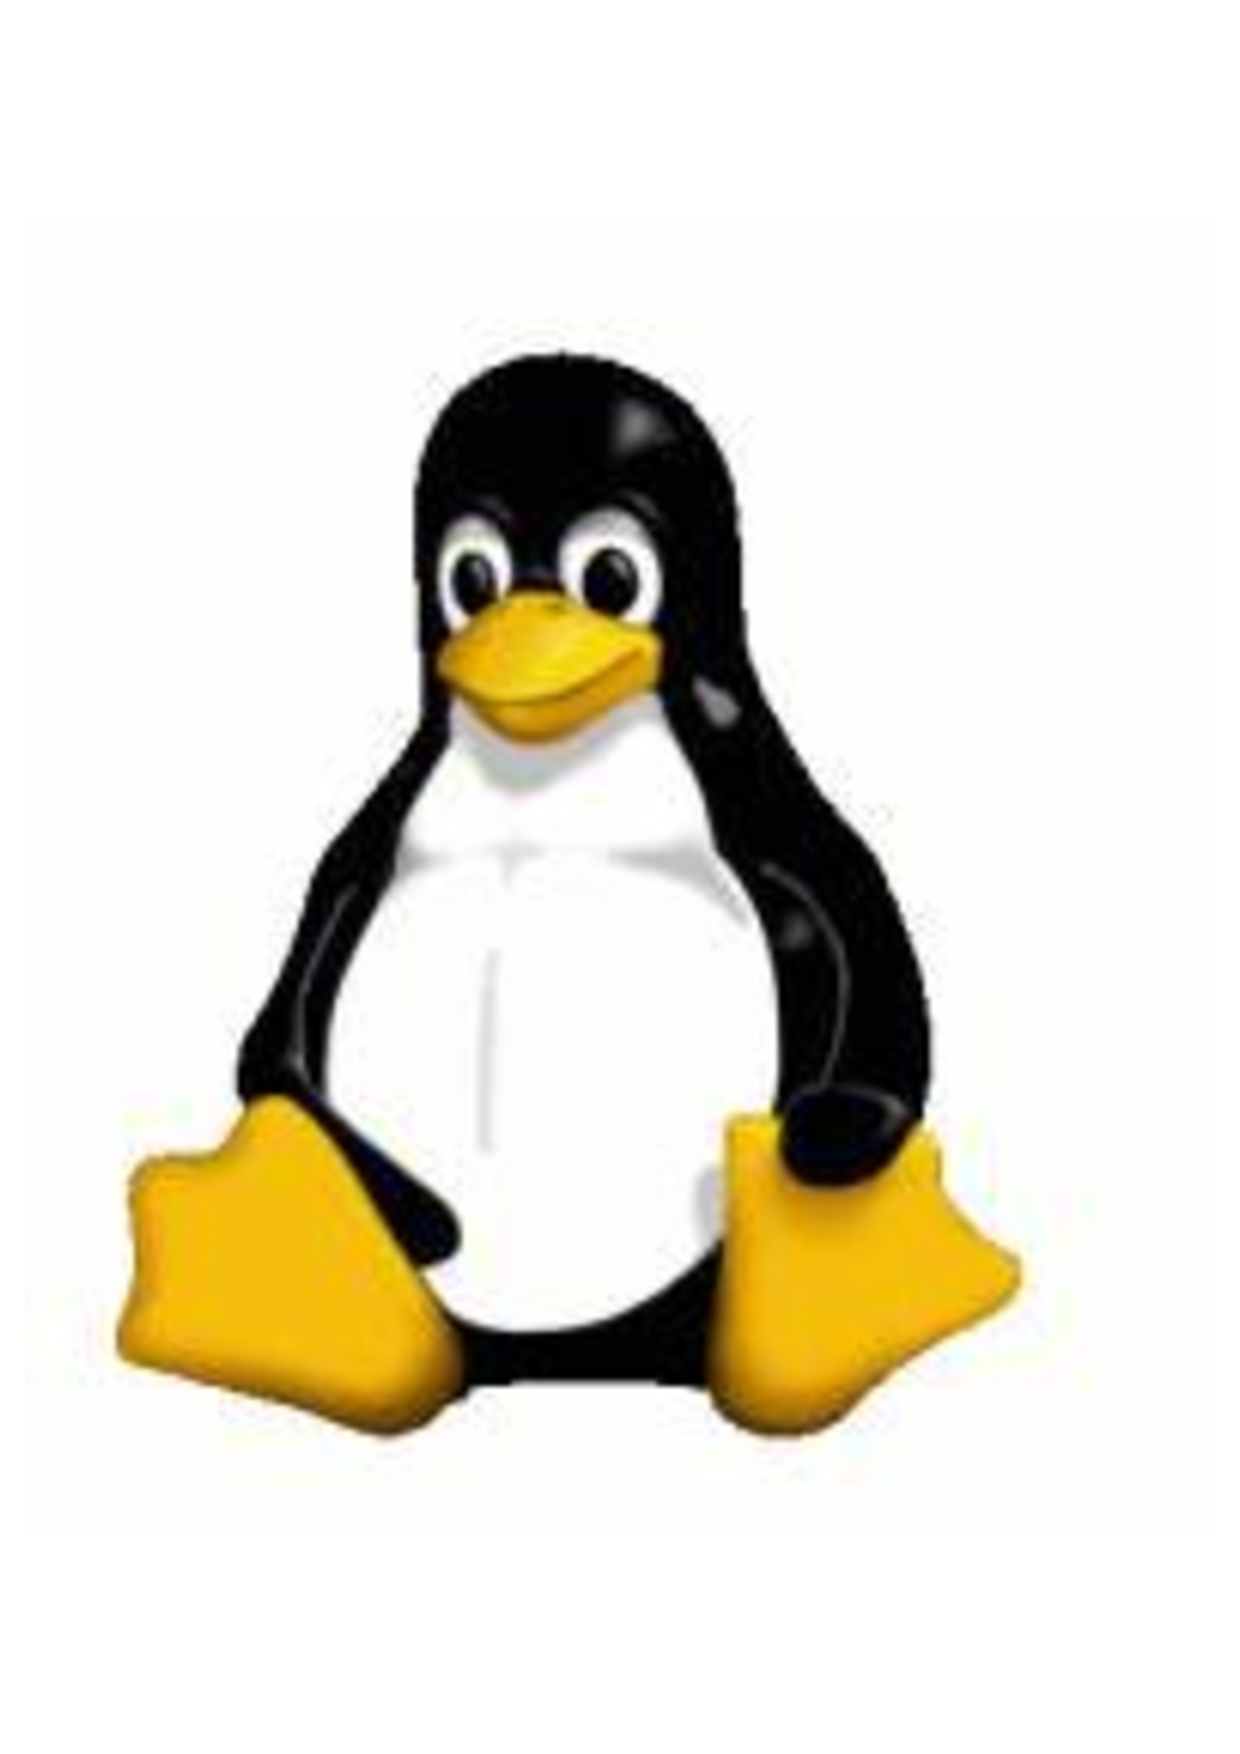
\includegraphics[scale=0.25]{Images/penguinOriginal.pdf}} &
    \onslide<2->{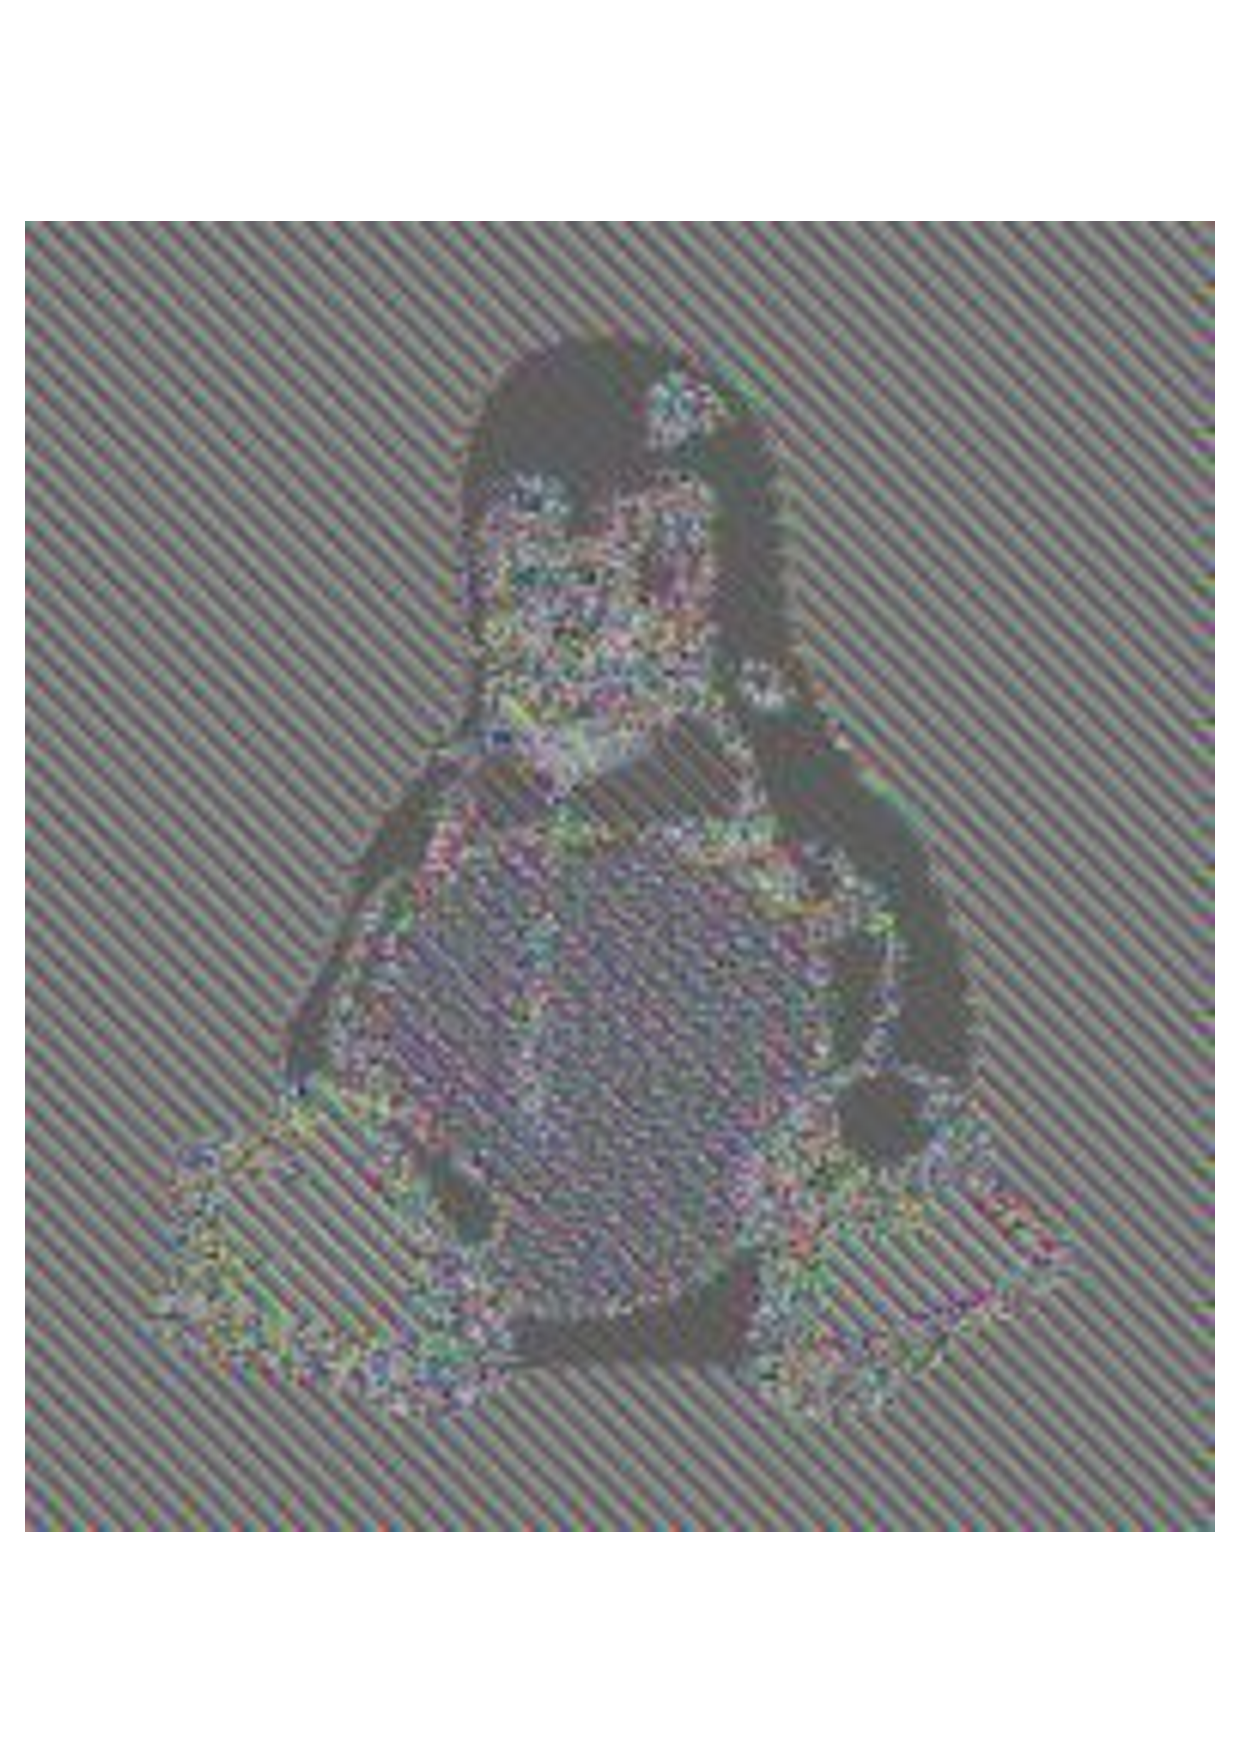
\includegraphics[scale=0.25]{Images/penguinECB.pdf}} \\[-2em]
    \onslide<1->{Original image} &
    \onslide<2->{Image encrypted using ECB mode} \\
  \end{tabular}
  \pause
     
\end{frame}

\begin{frame}{Cipher-block chaining (CBC) mode: encryption}
  \vspace{-0.5cm}
  \begin{center}
  \begin{tabular}{l}
    \noindent
    $(E, D)$ a block cipher that manipulates blocks of size $\ell$.\\
    %\hspace{-0.9cm}
    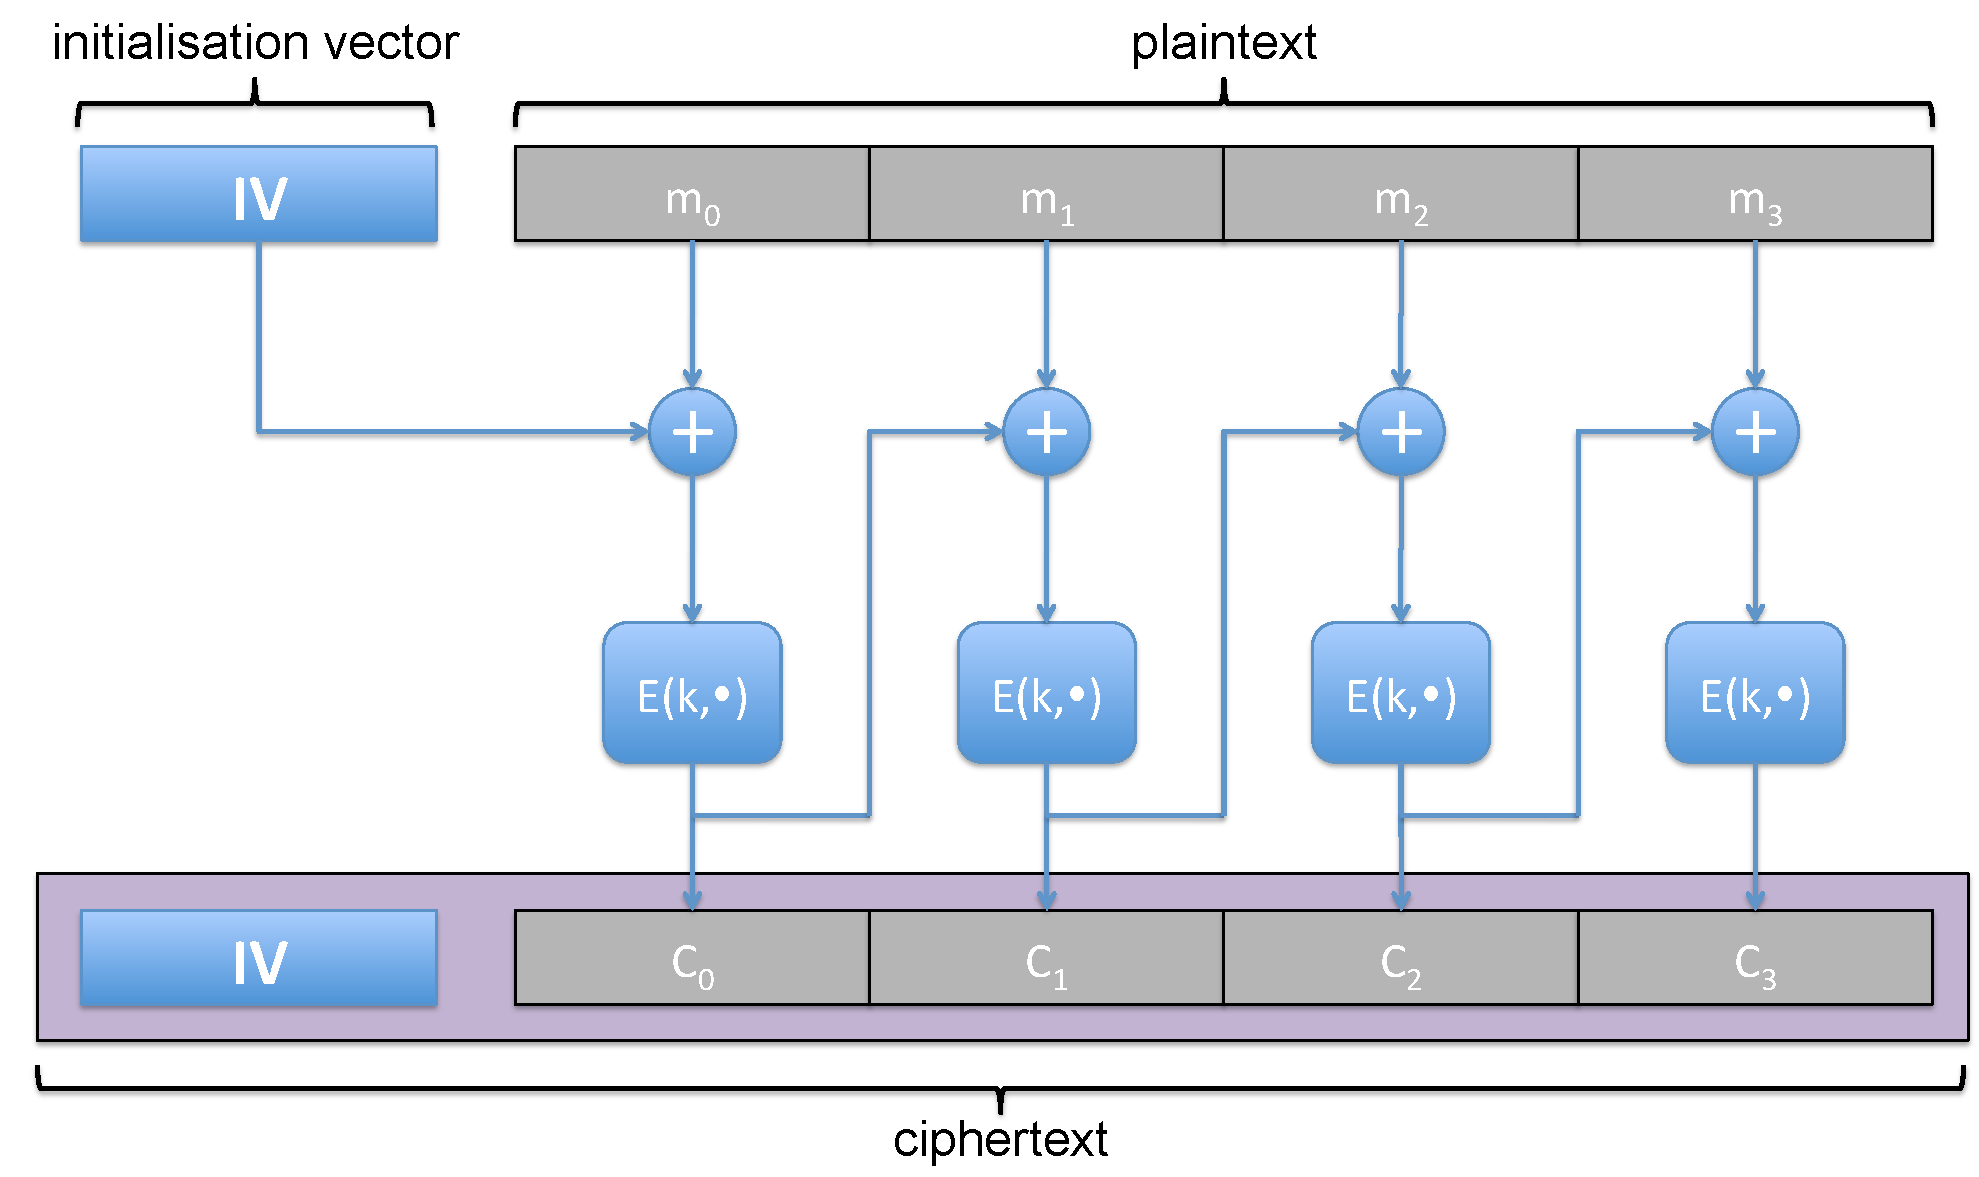
\includegraphics[scale=0.32]{Images/CBCenc.pdf} \\
    IV chosen at random in $\{0, 1\}^\ell$
  \end{tabular}
\end{center}
  

\end{frame}

\begin{frame}

  \frametitle{Cipher-block chaining (CBC) mode: decryption}
 \vspace{-0.5cm}
\begin{center}
  \begin{tabular}{l}
    %\hspace{-1.2cm}
    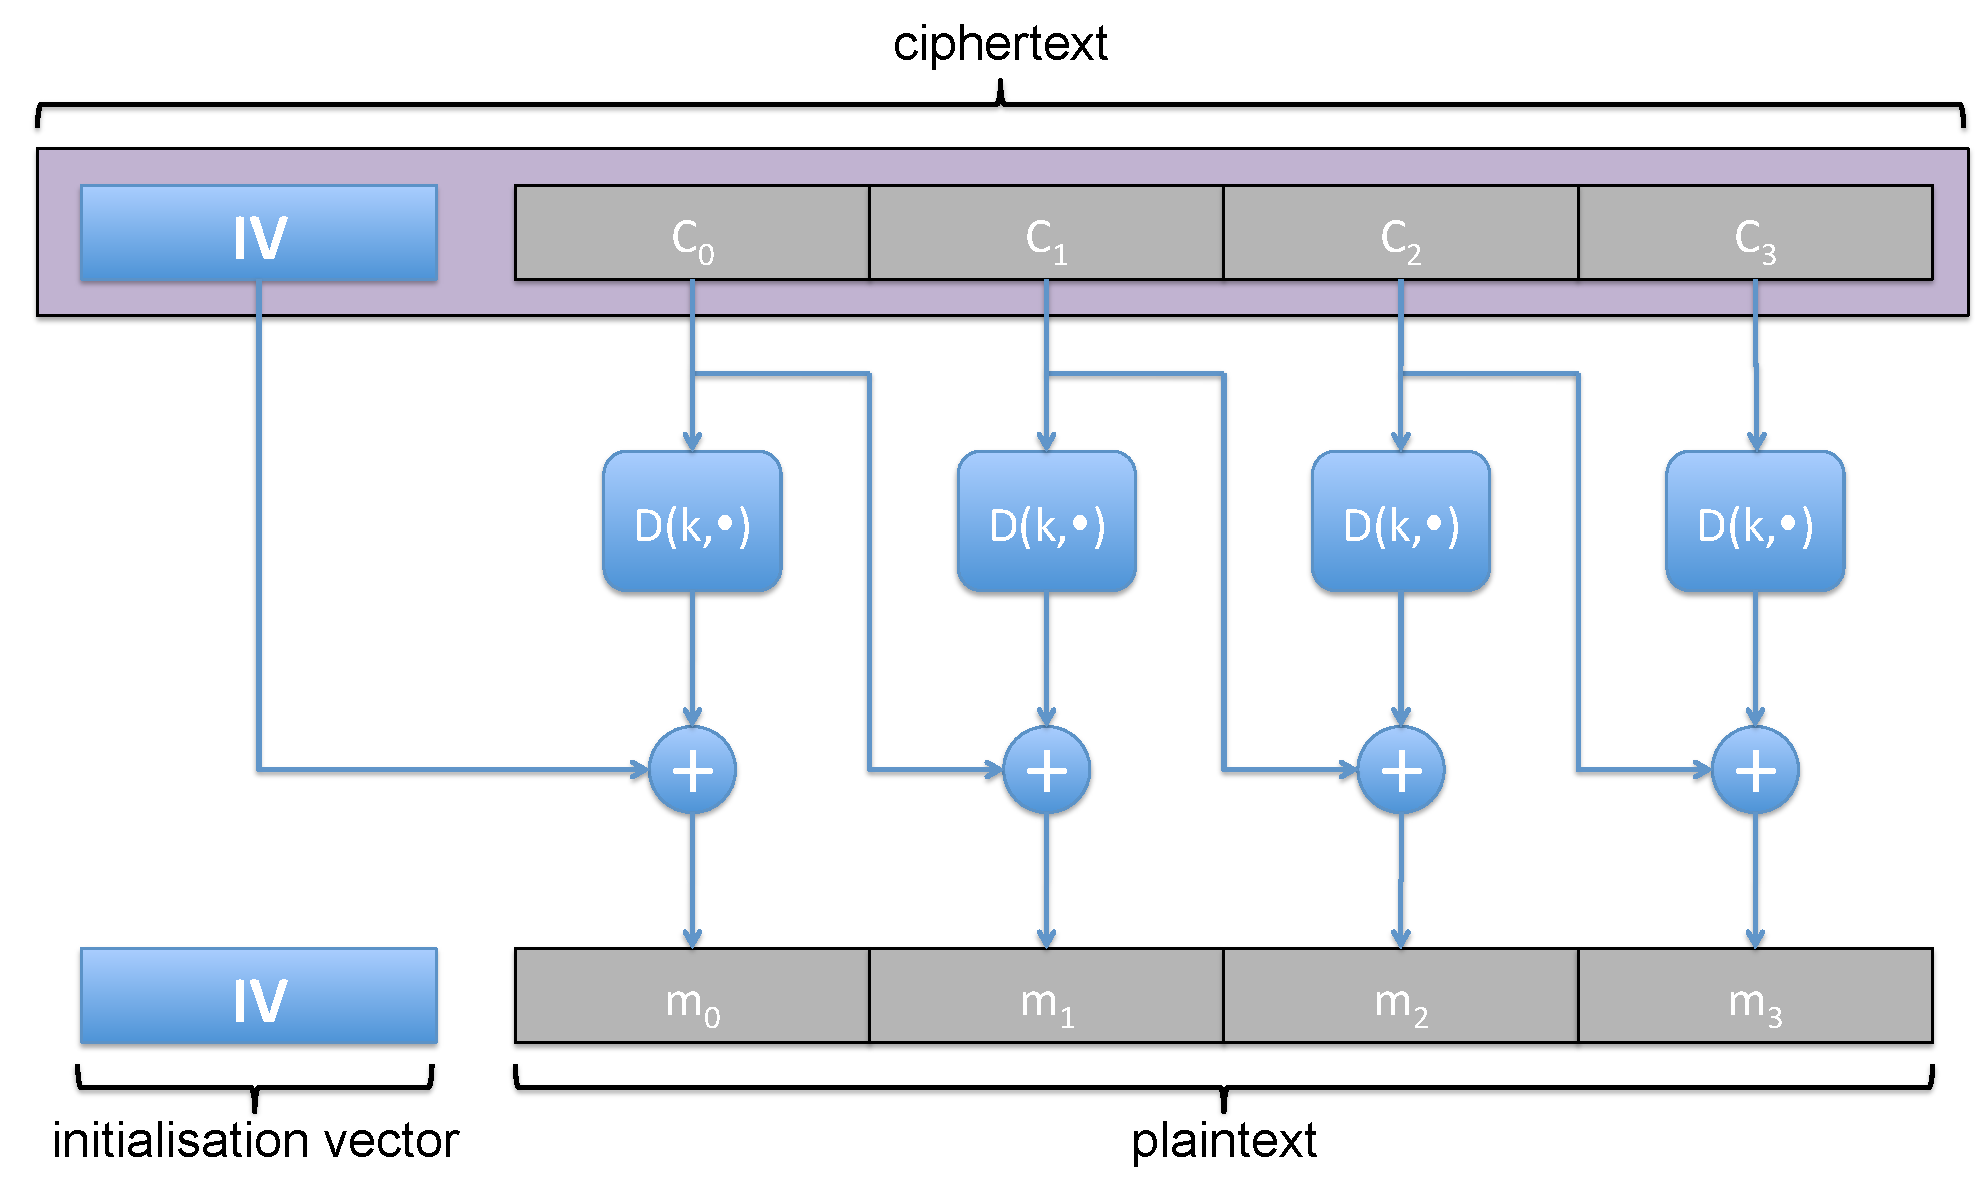
\includegraphics[scale=0.35]{Images/CBCdec.pdf}
  \end{tabular}
\end{center}

\end{frame}

\begin{frame}
  \frametitle{Sony PlayStation}

  \begin{columns}
    \begin{column}{2in}
      \begin{itemize}
      \item<2-> Prevent games being copied
      \item<3-> CD \& full disk encryption
      \item<4-> Users can read and write on dedicated areas of disk
      \item<5-> Games loaded in read only area of disk
      \item<6-> With CBC encryption need to encrypt/decrypt whole disk to access a game
      \item<7-> Sony PS used ECB full-disk encryption
      \item<8-> Hardware controlled user access to data
      \end{itemize}
    \end{column}
    \begin{column}{2in}
      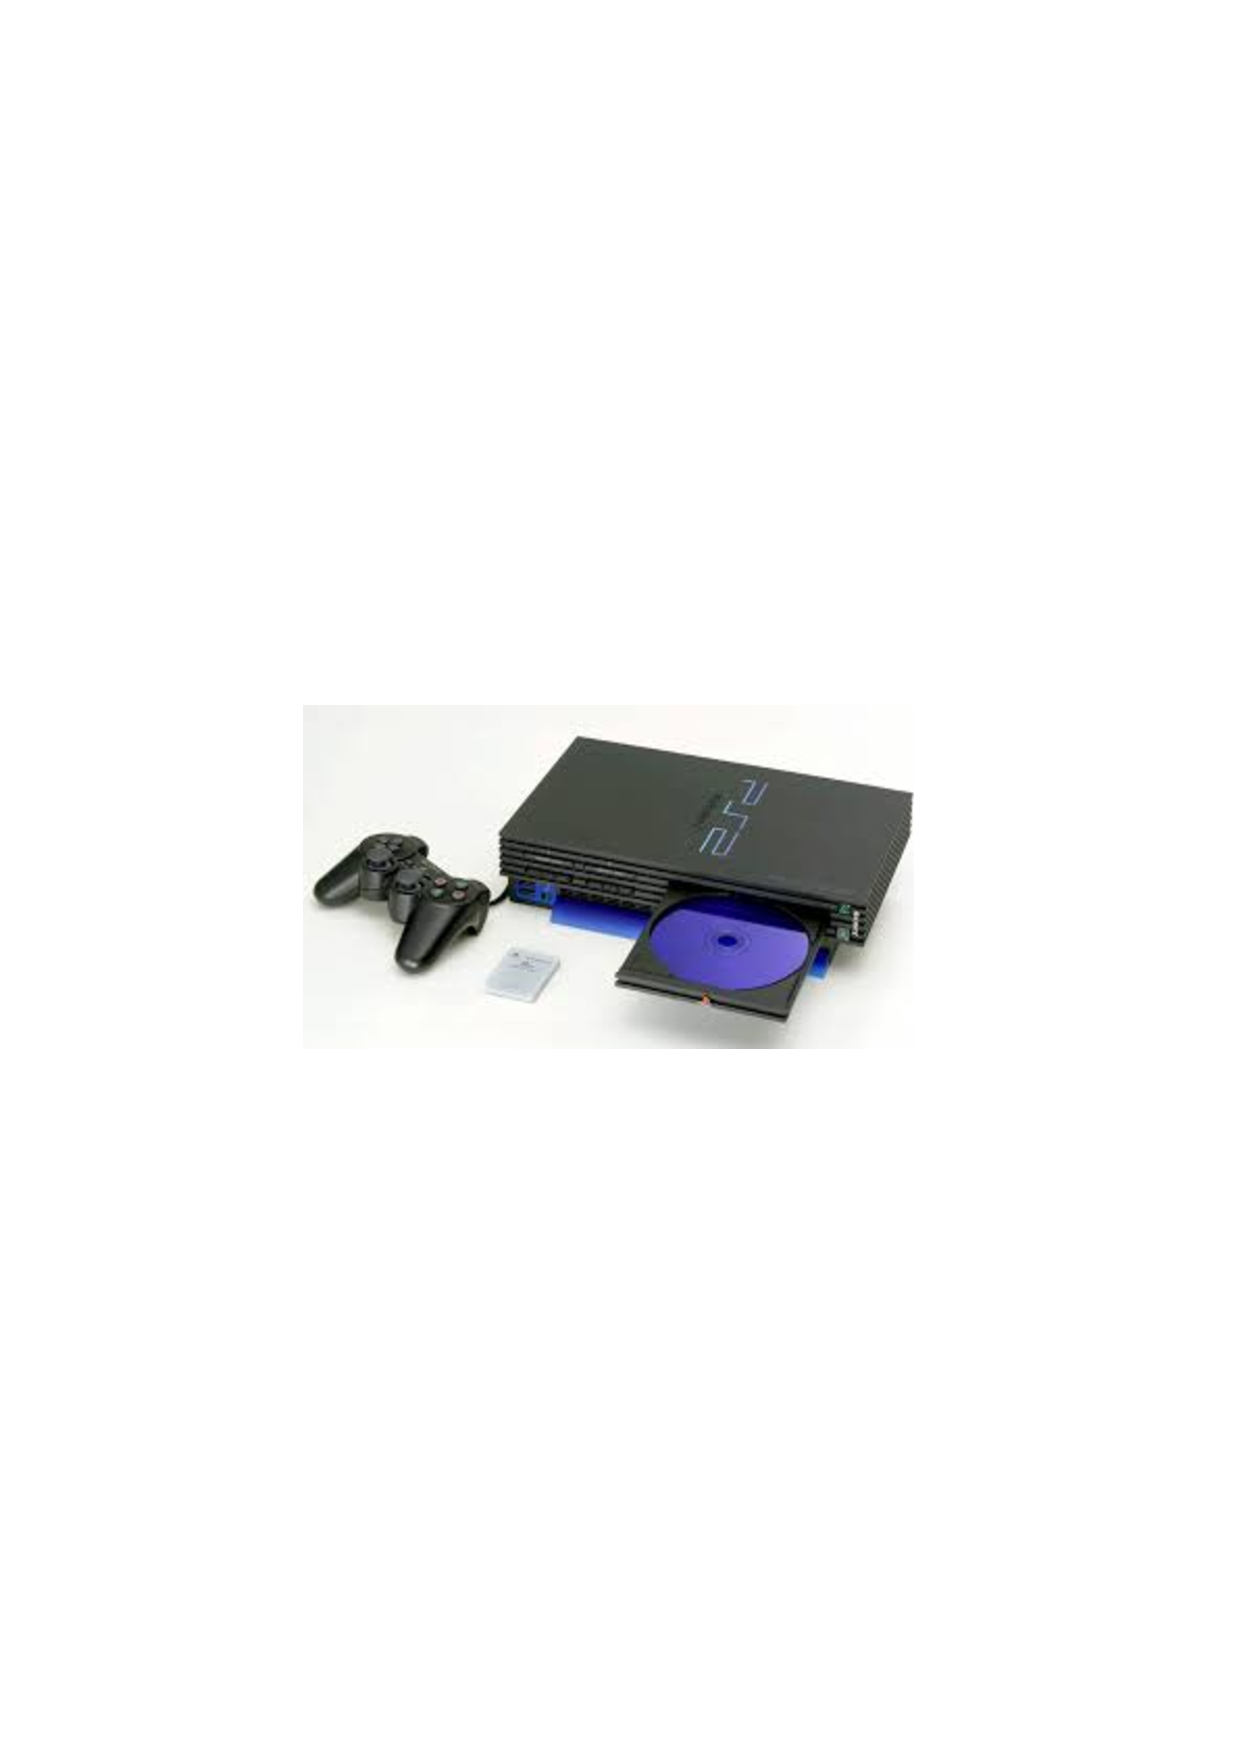
\includegraphics[scale=0.5]{Images/ps2.pdf}
    \end{column}
  \end{columns}
\end{frame}

\begin{frame}
  \frametitle{Sony PlayStation disk encryption attack}
  \begin{itemize}
  \item<1-> Remove disk and make copy
  \item<2-> Put disk back in PlayStation
  \item<3-> Copy a file to the disk
  \item<4-> Remove disk and find area of disk that changed  (that is the user encrypted file)
  \item<5-> Copy target data to the user area
  \item<6-> Put disk back in PlayStation and ask for user data
  \item<7-> PlayStation decrypts the file and gives it to user
  \end{itemize}

  
\end{frame}

\begin{frame}

  \frametitle{Counter (CTR) mode}

  \bigskip{}

  \begin{tabular}{l}
    $(E, D)$ a block cipher that manipulates blocks of size $\ell$.\\
    \\
    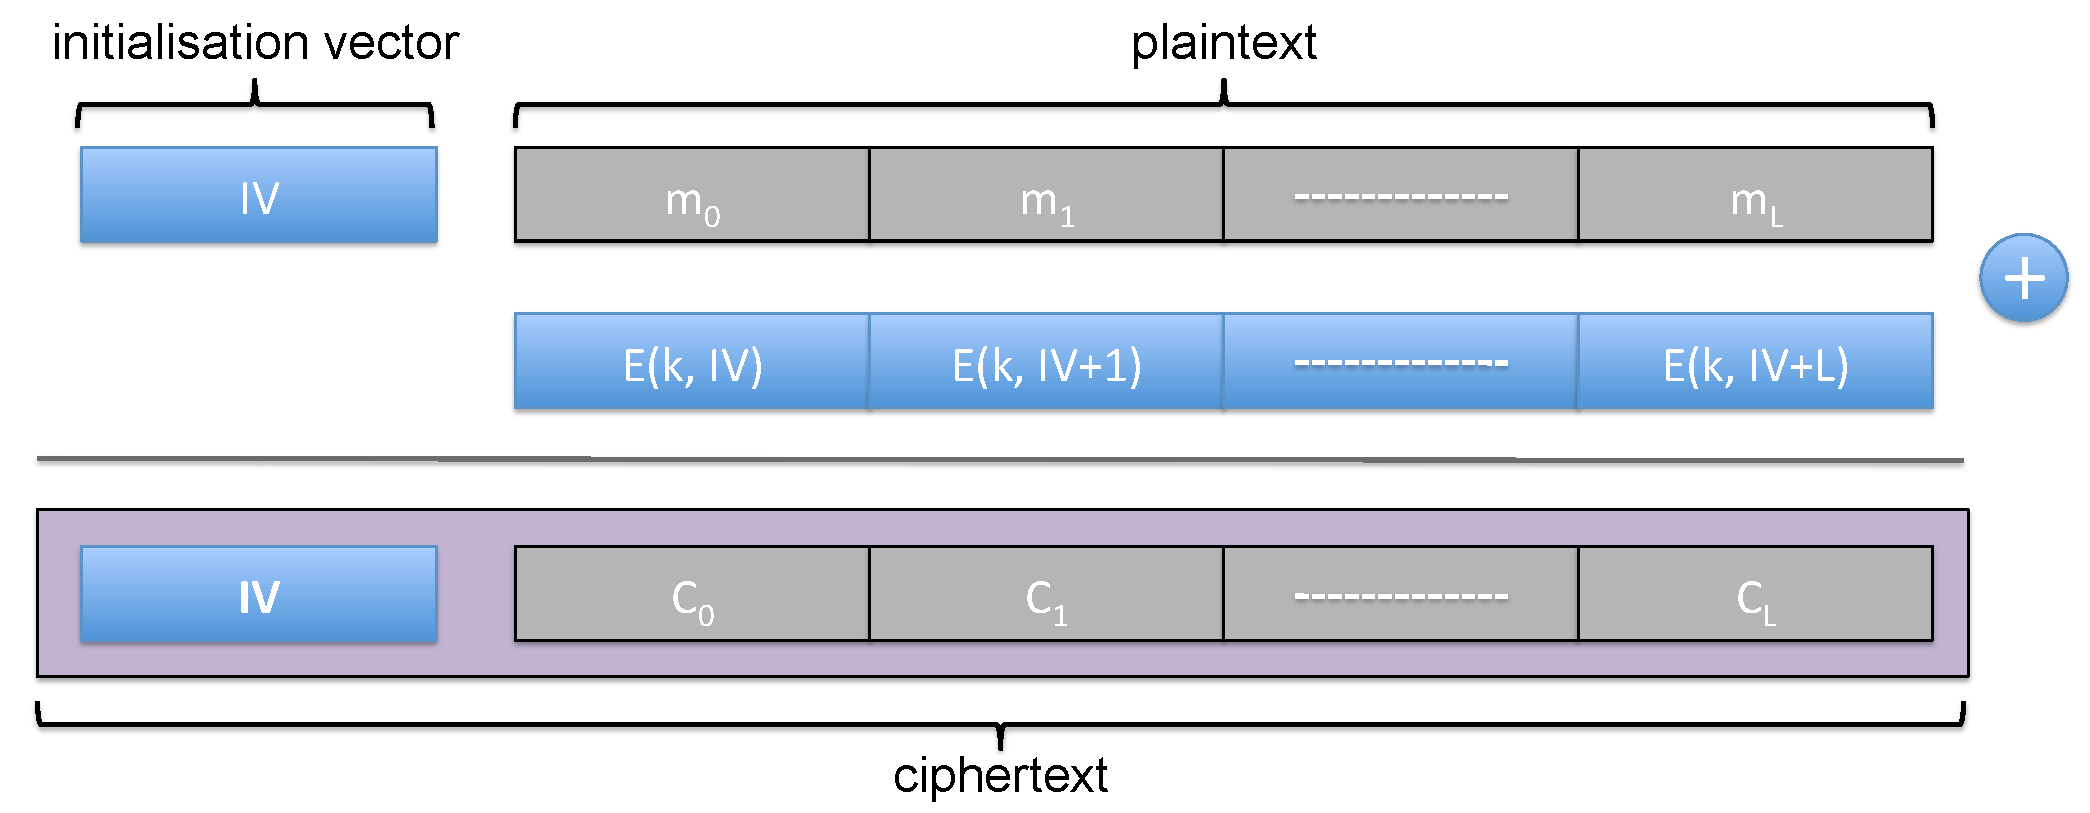
\includegraphics[scale=0.35]{Images/CTR.pdf} \\
    \\
    IV chosen at random in $\{0, 1\}^\ell$
  \end{tabular}

\end{frame}

\begin{frame}
  \frametitle{Block-size is also a problem!}
    \vspace{-0.5cm}
  \begin{itemize}
  \item Sweet32 - birthday attacks on 64-bit block ciphers in TLS and openVPN
  \item Attack due to block-size being too small
\end{itemize}
  \begin{center}
    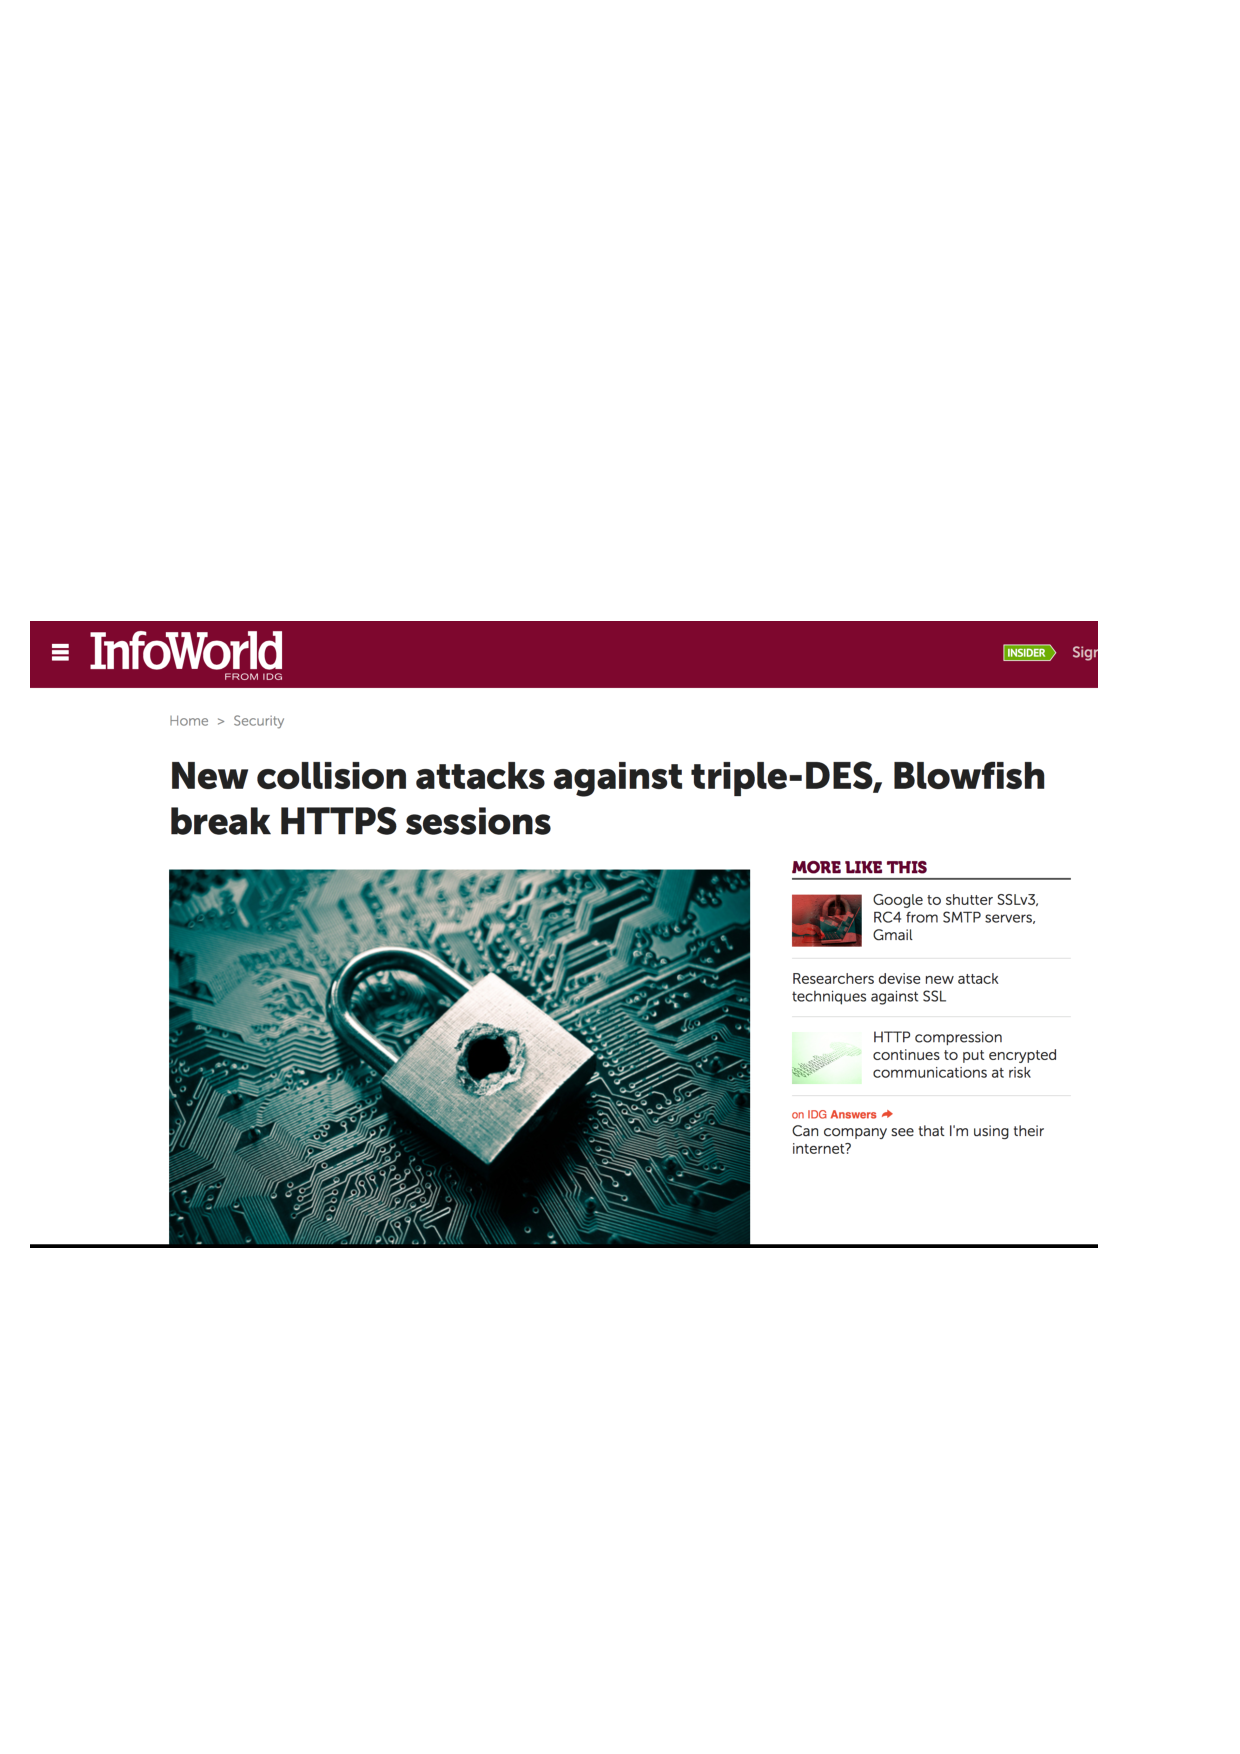
\includegraphics[scale=0.6]{Images/sweet32.pdf}
  \end{center}
\end{frame}

\begin{frame}{The key management problem}

  The confidentiality problem is now reduced to a key management problem:\medskip
  
  \begin{minipage}{0.525\linewidth}
    \begin{itemize}
    \item Where are keys generated?\medskip
      
    \item How are keys generated?\medskip
      
    \item How are keys shared?\medskip
      
    \item Where are keys stored?\medskip
      
    \item Where are the keys actually used?\medskip
      
    \item How are key revoked and replaced? 
    \end{itemize}
  \end{minipage}
  \begin{minipage}{0.45\linewidth}
      \begin{figure}[c]
        \centering
        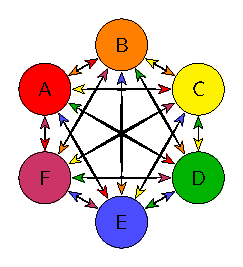
\includegraphics[scale=1]{Images/SKD.pdf}
        \caption*{One shared secret key per pair of users that want to communicate}
      \end{figure}
  \end{minipage}

  
\end{frame}

\begin{frame}{What we have learned on Symmetric Encryption}
  \vspace{-0.5cm}
  \begin{itemize}
  \item Frequency analysis as a cryptanalysis attack on classic encryption\medskip
  \item Importance of randomness in cryptography\medskip
  \item Stream ciphers
    \begin{itemize}
    \item simple and efficient symmetric encryption schemes 
    \item use a random IV to thwart two-time pad attacks
    \item subject to malleability attacks\medskip
    \end{itemize}
  \item Block ciphers - use AES not DES\medskip
  \item CBC mode is more secure that ECB but not resilient to packets loss\medskip
  \item CTR mode more secure than ECB and parallelisable \medskip
  \item Keep up to date with cryptanalysis advances and standards.\\  
  Modern symmetric encryption also guarantees authenticity \\$\rightarrow$ no malleability
  \medskip
  \item Do not implement crypto lightly - use public reference implementations
 \end{itemize}
\end{frame}


\end{document}